% Chinese reading edition corresponding to main.tex. Compile with XeLaTeX.
\RequirePackage[OT1]{fontenc}
\documentclass[letterpaper,journal]{IEEEtran}
\usepackage[UTF8,fontset=none,heading=false]{ctex}
\setCJKmainfont{FandolSong-Regular.otf}[BoldFont=FandolSong-Bold.otf,ItalicFont=FandolKai-Regular.otf,BoldItalicFont=FandolSong-Bold.otf,SmallCapsFont=FandolSong-Regular.otf]
\setCJKsansfont{FandolHei-Regular.otf}[BoldFont=FandolHei-Bold.otf]
\setCJKmonofont{FandolFang-Regular.otf}
\setmainfont{texgyretermes-regular.otf}[BoldFont=texgyretermes-bold.otf,ItalicFont=texgyretermes-italic.otf,BoldItalicFont=texgyretermes-bolditalic.otf]
\setsansfont{texgyreheros-regular.otf}[BoldFont=texgyreheros-bold.otf,ItalicFont=texgyreheros-italic.otf,BoldItalicFont=texgyreheros-bolditalic.otf]
\usepackage{amsmath,amssymb,cite,graphicx,booktabs,array,algorithmic,xcolor,tikz}
\usetikzlibrary{arrows.meta,positioning,fit,calc}
\usepackage[unicode,hidelinks]{hyperref}
\hypersetup{pdftitle={Next：以直接担保实现连续 UTXO 支付},pdfauthor={Lu Hengrun}}
\graphicspath{{figures/}{./}}
\renewcommand{\abstractname}{摘要}
\renewcommand{\IEEEkeywordsname}{关键词}
\renewcommand{\IEEEproofname}{证明}
\renewcommand{\figurename}{图}
\renewcommand{\tablename}{表}
\renewcommand{\refname}{参考文献}
\newtheorem{theorem}{定理}
\newtheorem{lemma}{引理}
\newtheorem{definition}{定义}
\newcommand{\Next}{\textsc{Next}}
\newcommand{\Hash}{\mathsf{H}}
\newcommand{\CAL}{\mathsf{CAL}}
\newcommand{\FUEL}{\mathsf{FUEL}}
\title{Next：以直接担保实现连续 UTXO 支付}
\author{Lu Hengrun\thanks{Lu Hengrun，大学。中文阅读版与英文修订稿对应。}}
\begin{document}
\maketitle
\begin{abstract}
持续支付要求收款方在先前交易仍待处理时复用已收到的价值。Next 通过注册担保组织，在未花费交易输出（UTXO）账本中支持这一操作。收款方在验证并记录某个输出及其法定人数签名证书（TXCer）后，即可请求后继付款，而公共执行异步进行。若已认证的来源缺失，委员会原子地执行该后继付款，并记录一项由来源发行者备付金支持的义务；该义务在来源执行时关闭，或在到期后通过备付金扣款关闭，赔付之后到达的来源向赔付方发行者回款。在固定成员与拜占庭故障下，我们证明了消费唯一性、包含隐藏证书在内的负债覆盖，以及延迟中性：对于来源全部执行的有限无冲突付款集合，每种成功的来源到达与赔付顺序最终得到的 CAL 最终持有人和备付金余额，都与无延迟执行相同。受限的资金来源修订保持完整区块身份。在单台 M4 Max 主机上（九个服务、内存状态、NoSync 钱包），100 跳链到达最后一个已认证收款的中位时间为 158.846\,ms，而每跳之间等待公共确认时为 65.204\,s；三次各 30,000 笔的运行含排空完成 1,750--1,887 笔/秒。九次回款运行（磁盘委员会）关闭了 21,600 笔付款，并回收全部 216 笔赔付。
\end{abstract}

\begin{IEEEkeywords}
UTXO 支付，支付担保，拜占庭容错，授权修复。
\end{IEEEkeywords}

\section{引言}
\label{sec:introduction}

在 UTXO 账本中，一笔支付花费的是先前某笔交易创建的输出。如果收款方必须等到该交易完成公共执行，支付链的每一跳都会增加一次确认延迟。设想 Alice 向 Bob 支付 100 CAL，Bob 再把收到的输出转给 Carol。要在公共执行之前转出这个输出，Bob 需要可验证的证据，证明其价值有资金支撑。如果 Bob 的支付先执行，账本就消费了一个 Alice 的交易尚未创建的输出，缺失的 100 CAL 需要一个明确的资金来源。无论 Alice 的交易先于 Bob 的到达、后于它到达，还是始终不到达，账务都必须保持正确。

基于证书的支付系统已经把收款方一侧的可用性与公共处理分离开来。FastPay 和 Zef 支持低延迟的认证支付，Sui Lutris 则针对不同类型的状态访问，把广播路径与共识路径结合起来~\cite{fastpay,zef,lutris}。支付通道协议依靠通道关系及其流动性实现快速转账~\cite{blitz,donner}。Next 处理的是原生账本上已认证支付的资金支撑问题，特别是所消费输出的源交易尚未执行的情形。源交易尚未执行的已认证输出，应当能够支撑一笔已公共执行的后继交易，并且应当由一个已提供备付资金的明确责任方对缺失的源交易负责。用户花费指定了消费路由的自有输出，注册组织为未解决的源交易提供支撑，交易对手无需预先注资的通道路径。

这里存在四个相互耦合的问题。第一，证书在公共登记之前就已流通，因此从公开登记的缺口开始记账会漏掉已经存在的承诺，而签名额度必须覆盖每一笔已认证支付的未清偿 CAL 负债，包括从未公开提交的支付。第二，源交易可能在委员会已经为其缺失的价值赔付之后才到达。迟到的源交易不能把同一笔价值既付给垫付它的担保人，又付给已经花掉它的收款方，否则延迟本身就会转移资金。第三，客户端可能持有源交易的材料却从不提交。签发组织的成员应能在赔付到期前补交已有的源交易，而赔付无需等待历史适配服务。第四，源交易一旦被赔付，读取已存储历史的人应当能够看出已消费的输入由哪份备付金提供资金。记录这一事实必须保持所有者授权、输出标识符以及后继交易所引用的承诺不变。仅有稳定的交易哈希，既无法界定也无法授权这样的修改。

Next 固定支付权利，并把未解决的源交易划归其直接签发组织负责。输出证书（TXCer）把一笔支付的输出绑定到一个明确的签发组织。收款方在验证并原子地记录输出及其 TXCer 之后，通过该输出指定的消费组织请求后继交易。该请求携带其直接输入的证书。所有者授权、花费状态、费用和资源限额则另行检查。

如果某个已认证的输入在公共创建状态中仍然缺失，委员会就原子地消费它，记录针对签发组织的直接义务，并创建子输出。在义务处于 Open 状态期间，子输出即为最终输出。承载该子交易的区块同时承载创建了被消费输出的那笔支付的证书。批准过该支付的签发组织成员，根据自己保存的批准记录重建该支付并补交，无需新的签名。如果源交易执行，义务即告履行。如果在期限之后赔付决定执行时源交易仍未出现，该决定就扣减签发组织的备付金，由它提供缺失的支撑，收款方不会得到第二次入账。该决定无需门限适配。之后到达的源交易在同一转换中偿还赔付它的签发组织，并且不为收款方创建第二个输出。当所有源交易最终都执行时，延迟只改变备付金的临时占用，本金的最终分配与无延迟时相同。

赔付决定本身就是一条关闭义务的公共记录。随后，历史表示命令在既有承诺之下，把已消费输入的资金引用替换为备付金引用。已存储的区块指明为该输入提供资金的备付金扣减，并且仍可对照其原始区块身份验证，因此读者能够在区块本身中核对指定历史输入的资金来源。钱包、同步和重放继续读取原始命令。我们把这一设计归纳为三项职责各异的贡献。

\noindent\textbf{C1：面向一轮续花的分层架构。}
我们把成员认证、收款方交付、证据复制和公共执行分离开来。成员在签名之前，原子地锁定输入并预留额度。一个并行认证轮产生一份 TXCer。INSTALL 在组织内复制完整材料，公共提交独立推进，二者均在后台进行。注册组织在组织内部和组织之间使用同一个证据接口，支付本金与担保人备付金保持分离。

\noindent\textbf{C2：有资金支撑且延迟中性的直接责任记账。}
我们定义原子的缺失输入转换及其关闭路径：由源交易履行、由公共赔付决定赔付、由迟到的源交易偿还。对于固定的输入与证书形态，请求的祖先证据不随转账深度增长。在固定成员的拜占庭模型下，我们证明唯一消费与资产守恒，并证明签名额度约束了证书（包括未公开提交的证书）的未清偿 CAL 负债。对于有限的、互不冲突且源交易全部执行的支付集合，到达与赔付的任意交错，最终得到的 CAL 持有和备付金余额都与无延迟执行相同。

\noindent\textbf{C3：证据驱动的源交易解决与保持身份的历史表示。}
我们让原签署者依据后继交易公开的证书补交源交易，并将赔付决定与门限适配分离。受限的历史表示命令没有经济效果，保持所有者授权、输出引用及完整区块身份（含分片集合头）不变。同一区块的命令共享受影响分片最终表示的适配，安装则直接推进到已提交的修订版本。对于固定的已决定槽位集合，最终区块体不依赖于命令如何分组。

我们在一台 M4 Max 主机上评估两个版本：续花与记账基线版本，以及增加了补交和独立赔付决定的 decision-first 版本。在基线版本上，100 跳链完成最后一次认证接收的三轮用时中位数为 158.846\,ms，而在各跳之间等待公共确认则需要 65.204\,s。三次各含 30,000 笔支付的运行（含后台排空）完成速率为 1,750--1,887 笔/秒，一个九次运行的矩阵关闭 21,600 笔支付，并偿还全部 216 次赔付。在 decision-first 版本上，三次运行的功能测试显示，被扣留的源交易无需赔付即可执行，而收款方的接收约需 14\,ms。在所有适配服务暂停的情况下，赔付与偿还仍然完成；六轮普通路径比较中，运行级接收 P50 和 P95 的范围相互重叠。第~\ref{sec:model} 节和第~\ref{sec:protocol} 节定义该设计，第~\ref{sec:security} 节和第~\ref{sec:evaluation} 节展开其安全性论证与评估。

\section{背景与相关工作}
\label{sec:related}

Next连接基于证书的连续续花、备付支撑的公共执行及授权历史修复。
最接近的工作已经在认证、抵押和受控编辑方面建立先例。
我们依据缺失资金来源的责任归属，以及责任落实过程中保持的付款与区块身份，界定Next的研究定位。

\subsection{基于证书的支付与执行}

FastPay通过拜占庭一致广播实现低延迟支付，
并支持由预充值资金支撑的主账本部署~\cite{fastpay}。
其可兑付性论证允许在相关入账转账尚未全部在本地确认时确认有效证书，
前提是补齐发送方先前转出付款的缺失证书。
兑付提供了一条基于证书从主账本资金池获取资金的路径。
Zef将可弃置账户与具有隐私性的可转让币相结合。
正常消费使用当前币证书及消费证据，而非完整的祖先交易历史~\cite{zef}。

Sui Lutris对归属特定所有者的对象采用广播执行，对共享对象的交互采用共识~\cite{lutris}。
Stingray通过拜占庭有界计数器和FastUnlock支持并发交易~\cite{stingray}；
其重叠额度与回收机制是与Next资源核算密切相关的先例。
其可交换事务工作负载所处理的争用问题，与每笔交易消费前序输出的支付链有所不同。
Next关注在资金来源交易执行之前，公共执行对经认证UTXO的消费，
同时登记由直接发行组织承担、具有资金保障的直接义务。
全部输出金额的预留与累计损失的保留，既计入已经公共登记的责任，
也计入隐藏证书所代表的承诺。

\subsection{通道与抵押担保}

Blitz使用pay-or-revoke替代通道支付中的两阶段提交，
Donner则构建应对Domino攻击的虚拟通道~\cite{blitz,donner}。
CryptoMaze提供部分付款不可链接的原子多路径通道支付，
同时避免在共享边上重复建立链下合约~\cite{cryptomaze}。
这些机制基于通道安排运行。
Next使用具有已注册消费路由和组织备付资金的原生账本，
因此交易双方既无需双边通道，也无需在彼此之间预先建立注入流动性的通道路径。

Snappy通过抵押支持的批准机制保护接受快速链上付款的商户。
可复用支付担保将隐私保护与可在规定时间窗口内重复使用的客户抵押相结合~\cite{snappy,reusable}。
Next则将用户付款本金与组织提供的额外担保资金分离。
其赔付关闭已执行子付款的缺失资金来源，而不再次向该子付款的收款人增加本金。

HyperService通过公共Network Status Blockchain与Insurance Smart Contract，
对跨链执行违约进行仲裁，并在资金层面撤销已提交交易的效果~\cite{web3}。
Next处理的是单个原生UTXO账本内不同的责任边界：
赔付结清发行组织的直接义务，同时保持已执行后继付款的本金效果。

\subsection{受控编辑与历史一致性}

变色龙哈希允许在同一摘要下存在经授权的替代消息，并为可编辑区块链设计提供基础~\cite{redactable}。
SDR研究去中心化的基于属性的编辑权限与动态委托；
Escaping将委员会选择和投票移至共识层之外，以减少修订等待~\cite{sdr,escaping}。
Reconstructing Chameleon Hash提出更强的不可区分性与抗碰撞性定义~\cite{reconstructCH}。
Next采用已有适配原语，由公共支付状态检查提供实施兼容替换的授权。

Reparo提供公开可验证的修复层，并可在修复状态时重新执行受影响的交易~\cite{reparo}。
Next固定付款授权和输出：公共修复命令对赔付进行核算，
历史物化则替换获准修改的资金来源表示，而不重新执行后继付款。
原始命令和后续修复仍构成经济重放历史。

RedactChain协调同块并发编辑冲突与预处理~\cite{redactchain}。
CDEdit使用可复用权限令牌，减少多次编辑中重复的令牌和密钥生成及验证工作~\cite{cdedit}。
Next的批处理在共享最终区块表示的同时，保留每项直接义务的资格、备付扣款和终态检查。
其完整区块身份由稳定区块头哈希与原始分片集头共同构成。
经公共提交的逻辑修订授权确切的替换正文；物理安装可直接推进到后续已授权修订。
这一设计将仅生效一次的经济赔付与表示更新的物理安装分离，
同时保持后继引用，并支持重放同一公共命令历史。

\section{系统模型与概述}
\label{sec:model}

\subsection{参与者、输出与证书}
\label{sec:model-participants}
\label{sec:model-certificates}

Next 运行原生 UTXO 账本。CAL 承载支付价值，FUEL 支付处理费用。用户授权消费输入并创建收款输出和找零输出的支付。已注册组织认证支付，并在公共备付账户中持有额外 CAL。用户保留本金所有权，但批准会锁定所选输入，阻止冲突花费。交易双方无需建立双边通道。费用通常使用付款人持有的最终 FUEL 输出；组织也可以授权费用赞助。

每个组织有四名固定成员和一个可替换的收集者。成员独立检查请求，在签名前记录输入锁与额度预留。收集者分发请求，将三个匹配签名汇集为法定人数证书（QC），自身不获得花费权限。TXCer 由该 QC 与经认证的支付摘要组成。独立委员会 $\mathcal C$ 包含四名权重相等的验证者，负责公开命令的排序与执行，需三票，并维护输出、备付与义务。

输出指定资产、金额、所有者和消费路由。快速支付的全部本金输入指向同一消费组织，由该组织认证这笔支付并发行新输出的证书。每个新输出的路由指定认证之后花费它的支付的组织。输出的\emph{来源}（亦称父）是创建它的交易；\emph{后继}（亦称消费方或子）花费该输出。子输出指消费方创建的输出。每笔支付还携带 Intent，用于跨组织标识同一付款人的一次操作。

输出标识符 $x$ 绑定网络、创建交易和输出位置。花费以 $(x,i)$ 索引，普通输出的 $i=0$。TXCer 绑定网络、交易身份、发行方、配置、纪元、规则、输出承诺与金额，以及准入 grant。三个不同成员签名覆盖同一事实 $c_T$。输出正文可以单独交付；接收方在记录输出之前检查承诺、位置与所有权。表~\ref{tab:model-notation} 汇总符号。

\begin{table}[!b]
\caption{主要符号。}
\label{tab:model-notation}
\centering
\begin{tabular}{@{}p{0.23\columnwidth}p{0.69\columnwidth}@{}}
\toprule
符号 & 含义 \\
\midrule
$G,\mathcal C$ & 担保组织与公共委员会 \\
$T,c_T$ & 支付及其经认证的摘要事实 \\
$(x,i)$ & 输出标识符与花费实例 \\
$g,B_g$ & Grant 与累计授权额 \\
$a_T,p_T,\mathsf{Rec}_T$ & CAL 输出总额、赔付总额（毛额）与已偿还的赔付额 \\
$\mathcal O_x,\mathcal D_x$ & 针对缺失输出的直接义务及其不可变的赔付决定 \\
$(H_b,P_b)$ & 稳定区块哈希与原始 part-set 头 \\
$\rho_\ell,\rho_p$ & 已提交的逻辑修订与已安装的物理修订 \\
\bottomrule
\end{tabular}
\end{table}

\subsection{故障与状态假设}
\label{sec:model-assumptions}

\noindent\textbf{故障与密码学。}
对手在整个执行期间静态地至多腐蚀每个组织的一名成员和一名委员会验证者；用户与收集者的行为任意。诚实参与者共享网络配置、创世、规则与组织注册表，每条路由指定一个活动配置和一个消费锁域。签名不可伪造，规范摘要与原始区块承诺具有绑定性，消息可被任意延迟。

\noindent\textbf{状态。}
诚实的签名状态是原子的，且从不被遗忘或回滚。成员签名之前，其批准记录了该请求的支付、准入向量和直接输入证书；法定人数证书不属于其中。公开执行是确定性的并以原子方式提交，跟随者应用经认证的连续区块，同时更新状态与游标。赔付与表示读取原始区块及其元数据，因此正确的委员会副本在每个存在未结义务或待表示的已决定槽位的高度上都保留这两者。

\noindent\textbf{适配与进展。}
可信的离线 dealer 生成三取四适配密钥，并向四名公共委员会验证者各分发一份。相同的静态、至多一名 Byzantine 假设适用于这些持有者。适配需要三份有效贡献；三名响应的诚实验证者足以提供这些贡献。任何适配后的正文仍必须由已提交的命令授权。进展需要响应的诚实参与者、可用的证据、充足的费用与资源，以及公平的交付与调度。实验用的内存配置仅在进程运行期间保持状态原子，且每次运行都从全新的创世开始。

\subsection{认证续付}
\label{sec:model-example}

考虑 Alice 的支付 $T_A$：消费一个最终的 100 CAL 输入，创建向 Bob 支付的 40 CAL 输出 $x$，并返回 60~CAL 找零。其输入指向 $G_A$，而 $x$ 指向 $G_B$。$G_A$ 认证 $T_A$，并始终是对 $x$ 负责的发行方。Bob 在记录到账之前，对照 $x$ 的正文、承诺、位置、所有权与可信配置检查证书。

Bob 随后可以授权 $T_B$，花费 $x$ 向 Carol 支付 40 CAL，并在 $T_A$ 公开执行之前请求 $G_B$ 认证。$G_B$ 根据自身的输入锁、Intent 记录、费用与可用资源检查 $T_B$，法定人数批准后便发行 $T_B$ 输出的证书。$G_A$ 和 $G_B$ 可以是同一组织。证书为 Bob 的请求提供认证证据；针对缺失 $x$ 的公开义务在 $T_B$ 成功执行时产生。接收方核验与原子本地记录完成快速路径，完整材料复制与公开提交在后台推进。图~\ref{fig:architecture} 展示这两笔支付。

\begin{figure*}[t]
\centering
\begin{tikzpicture}[x=1cm,y=1cm,font=\footnotesize,
  box/.style={draw=black!55,rounded corners=2pt,align=center,minimum height=1.0cm,text width=2.6cm,fill=white},
  flow/.style={-{Stealth[length=2mm]},thick,draw=blue!60!black},
  bgflow/.style={-{Stealth[length=2mm]},draw=black!65,dashed},
  lab/.style={font=\scriptsize,align=center,fill=white,inner sep=2pt}]
\node[box,text width=1.9cm] (sender) at (0,0) {付款方钱包\\\textbf{授权付款}};
\node[box,text width=3.3cm,fill=blue!4] (org) at (4,0) {消费裁决组织\\4名独立成员\\\textbf{3份匹配签名}};
\node[box,fill=blue!4] (wallet) at (8.8,0) {收款方钱包\\验证并记录TXCer\\\textbf{可发起后继付款}};
\node[box] (next) at (13,0) {后继付款\\相同或其他\\已注册组织};
\draw[flow] (sender) -- node[lab,above]{交易} (org);
\draw[flow] (org) -- node[lab,above]{输出 + TXCer} (wallet);
\draw[flow] (wallet) -- node[lab,above]{直接证据} (next);
\node[box,text width=3.3cm,fill=green!4] (comm) at (4,-3) {公共委员会\\\textbf{执行子付款}\\单次消费；记录直接缺口};
\node[box,fill=green!4] (resolve) at (8.8,-3) {等待资金来源\\来源到达后\\关闭直接义务};
\node[box,fill=orange!6] (repair) at (13,-3) {授权修复\\备付扣款 + 修订\\来源迟到：偿还原组织\\后台历史物化};
\draw[bgflow] (org) -- node[lab,right]{公共提交} (comm);
\node[lab,left] at (2.1,-1.25) {后台成员证据安装（INSTALL）\\在组织内部\\复制完整证据};
\draw[bgflow] (comm) -- node[lab,above]{直接\\义务} (resolve);
\draw[bgflow] (resolve) -- node[lab,above]{到期时\\仍未成立} (repair);
\node[align=center,font=\scriptsize,text=black!75] at (8.6,-4.5) {资金来源的落实保持已授权输出与后继引用不变。\\钱包与成员跟随经认证的公共区块更新状态；无需委员会逐笔通知。};
\end{tikzpicture}
\caption{Next中的连续支付与资金来源的公共落实。实线箭头表示收款人的续花路径，虚线箭头表示后台工作。每笔后继付款均需独立授权；尚未落实的资金来源由其直接发行组织承担责任，而不是作为等待祖先交易的要求向后传播。历史修复由后续公共命令授权；赔付后来源成功执行时偿还原赔付组织，不再向收款方重复入账。}
\label{fig:architecture}
\end{figure*}


\subsection{公开消费与来源闭合}
\label{sec:model-contract}

若 $T_A$ 先于 $T_B$ 执行，$T_B$ 消费 $x$ 时它已是最终公开输出，无需缺失来源义务。若 $T_B$ 通过公开检查并先执行，委员会原子地记录 $x$ 的消费、创建 $T_B$ 的最终输出，并登记针对 $G_A$ 的 40 CAL 义务。该义务仍为 Open 时，Carol 已可按普通最终输入规则花费自己的输出；她的下一笔支付仍须通过指定组织的认证与准入。携带 $T_B$ 的区块也公开 $T_A$ 的证书。$G_A$ 的原签名成员可将该证书与保留的批准材料组合，无需新的所有者或成员签名即可重新提交 $T_A$。

若 $T_A$ 在义务处于 Open 时执行，便履行义务并关闭缺口。即使截止期已过，只要赔付尚未执行，仍可如此处理。由公开区块时间锚定的截止期到达后，入块且有效的赔付决定可改为从 $G_A$ 备付金扣除 40~CAL，关闭缺口。$T_B$ 的本金效果保持不变。每项输入义务的关闭更新 $T_B$ 的费用记账；其托管在全部输入义务解决后结清。

若 $T_A$ 在赔付后执行，它消费自己的输入，向同一备付账户偿还 40~CAL，而不重新创建 $x$。未消费的找零正常创建，赔付决定保持记录。若 $T_A$ 始终不执行，已赔付的 40~CAL 就成为 $G_A$ 的损失。若 $T_A$ 和花费 $x$ 的合法后继均未执行，Bob 的证书不提供仅凭证书的兑付或无条件退出；等待本身也不会产生该权利。表~\ref{tab:model-contract} 给出各阶段的保证。

\begin{table}[!t]
\caption{各阶段的服务契约。}
\label{tab:model-contract}
\centering\small
\begin{tabular}{@{}>{\raggedright\arraybackslash}p{0.24\columnwidth}>{\raggedright\arraybackslash}p{0.69\columnwidth}@{}}
\toprule
触发事件 & 已成立的状态 \\
\midrule
验证后到账 &
发行方的 QC 绑定输出及其所有者。收款人可以请求后继，
后继仍须通过自身的准入检查。到账本身不产生公共赔付义务。 \\
公开消费缺失的认证输出 &
成功执行原子地消费输入、登记直接发行方的义务并创建子输出。
授权、费用、消费状态、Intent 和覆盖均须通过公开检查。在给定故障与状态模型下，合法证书具有充足的 CAL 授权（定理~\ref{thm:security-coverage}）。 \\
责任闭合 &
来源执行履行义务；否则，入块且有效的到期后决定扣减发行方
CAL 备付。之后到达的来源偿还该备付，不向收款人重复入账。
截止期本身不保证闭合已经完成。 \\
\bottomrule
\end{tabular}
\end{table}

\subsection{签名容量、公共覆盖与缺口}
\label{sec:model-layers}

三个量分别记录该示例的不同阶段。签名容量限制各成员的批准。公共覆盖跟踪已登记证书的输出。开放缺口记录已经公开消费的缺失输出价值。发行方备付账户提供通过赔付关闭缺口所需的 CAL。

每名批准 $T_A$ 的成员预留 100~CAL，同时覆盖 $x$ 与 Alice 的找零。这项预留保护可能在公开登记之前就已流转的承诺。$T_B$ 首次消费缺失的 $x$ 时，委员会登记 $T_A$ 全部 100~CAL 输出的覆盖，但仅建立 40 CAL 缺口。其余 60~CAL 仍被覆盖。登记不改变备付余额；随后的赔付才扣除 40~CAL。成员在认证 $T_A$ 已成功执行后恢复自己记录的 CAL 容量；仅发生赔付时，该容量仍被预留。

累计授权为 $B_g$ CAL 的 grant $g$ 给予每名成员 $\lfloor2B_g/3\rfloor$ 签名容量，并在其本地执行 Worker 间划分。Worker 是带资源切片的内部处理单元，不是额外的验证者。每名批准成员预留 $a_T$，即包含找零的全部 CAL 输出值。这些重叠的签名容量不会增加支持资金。诚实签名者保留未结证书责任对应的预留，使覆盖证明能够统计尚未公开的证书。创世时按支持账户检查汇总 grant；授权补资同时提高余额与 grant，授权额不减少。

任何客户端都可以收集批准，而不获得花费或费用赞助权限。成员批准前原子检查 Intent、输入锁、费用、grant 与全部适用资源切片。容量不足时拒绝该次批准，不提交变更，也不返回签名。重试已有且未失效的批准不增加预留。新请求仍需法定人数具有可用容量。局部或被放弃的批准可能占用容量而未形成证书，因此备付仍有资金时也可能停止新认证。停止签发不撤销证书，也不解除输入锁。

组织保留本地 Intent 记录，公开执行则对同一操作至多接受一笔交易。因此，具有相同 Intent、输入互不相交的两笔交易可能被不同组织分别认证，但至多一笔公开执行。未执行的落败交易即使已发生赔付，也保留其签名预留。耗尽额度可阻止路由到该组织的其他用户支付，包括花费最终输出的支付。FUEL 支出与被锁来源输入是不同的成本；费用赞助不会把直接发行方的 CAL 责任转移给费用支付者。

实现没有付款人级 CAL 准入上限，也没有跨收集者的未完成请求上限；费用赞助策略与网关并发限制并不提供这两者。第~\ref{sec:security-composition}~节给出持续准入所需的工作负载与容量条件，并约束发行方未偿还赔付净额。

\subsection{经济闭合与历史记录}
\label{sec:model-records}

赔付后，$T_B$ 的原始输入仍指向 $x$，即 $T_B$ 执行时接受的对象。本地归档操作者可能需要报告 $G_A$ 的备付垫付，并导出在原输入位置显示该垫付的记录。由决定授权的修复把备付扣款记入该输入，同时保持支付授权、输出引用和原完整 BlockID：区块头哈希与原 part-set header。

在已验证并执行的公开前缀 $H$ 上，读取者使用状态 $V_H$ 的一个读事务及保留历史，取得授权表示、永久决定和当前义务状态。偿还之后，备付引用仍记录历史垫付。普通决定索引可以回答同样的经济问题；修复进一步把扣款引用置于与原完整 BlockID 相容的正文中。逻辑修订与物理安装分别推进，重放使用保留的原始命令。修复需要已提交的赔付决定；赔付与偿还无需等待适配或安装。

表~\ref{tab:model-states} 区分这些状态。例如，义务已为 Compensated 时，输入仍可能是 \texttt{OriginalFunding}，且尚未安装物理修订。第~\ref{sec:protocol-reader}~节规定本地读取与导出接口。


\begin{table}[!t]
\caption{相互独立的状态维度。}
\label{tab:model-states}
\centering\small
\setlength{\tabcolsep}{3pt}
\begin{tabular}{@{}p{0.24\columnwidth}p{0.70\columnwidth}@{}}
\toprule
维度 & 含义 \\
\midrule
公开支付 &
成功执行（\texttt{Settled}）创建最终输出，即使仍有未结输入义务（\texttt{Pending}）。迟到来源执行时，其每个已获赔付输出的对应金额返还原赔付备付账户，该输出不再被重新创建。 \\

直接义务 &
Open$\to$Fulfilled，或 Open$\to$Compensated$\to$Recovered。
Compensated 表示赔付；Recovered 表示随后的偿还。
赔付决定持续存在。 \\

逻辑表示 &
$V_H$ 中的修订决定该槽位。
\texttt{OriginalFunding} 并不意味着不存在赔付。
\texttt{ReserveFunding} 记录一次历史垫付，并在偿还之后仍然保留。 \\

物理安装 &
$\rho_p$ 记录已安装的区块存储版本。
安装进度不决定 $H$ 处的逻辑答案，也不改变经济状态。 \\
\bottomrule
\end{tabular}
\end{table}


%% ===== zh-protocol.tex =====
% 本节片段对应英文稿 protocol.tex。
% 需要 amsmath、amssymb 和 algorithmic。
% 两个伪代码块使用 IEEEtran 的图浮动体，而不是 algorithm 浮动体。

\section{协议设计}
\label{sec:protocol}

Next 认证固定的付款授权和输出，同时允许其来源保持未决。收款方在授权后继付款时把 TXCer 用作证据。公共执行原子地消费缺失的已认证输入，并记录其直接发行者义务。经授权的修复把义务的经济关闭与一个精确的替换资金表示一起提交。历史安装在该提交之后进行，且从不重新执行该付款。

\subsection{身份、认证与交付}
\label{sec:protocol-certification}

令 $K_T$ 表示编码后的付款正文与输入声明，$\mathbf{C}_T$ 表示其输入承诺，$\Sigma_T$ 表示其输出摘要：
\begin{equation}
  \begin{aligned}
    K_T &= \operatorname{Encode}(T.\mathsf{Body},T.\mathsf{Claims}),\\
    \mathsf{id}(T) &= H(\texttt{TX\_V3},K_T,\mathbf{C}_T),\\
    c_T &= H(\texttt{DIRECT\_CERT\_V3},\operatorname{Encode}(\Sigma_T)).
  \end{aligned}
  \label{eq:protocol-identities}
\end{equation}
所有者签名认证 $\mathsf{id}(T)$，但不进入其计算。每个输出标识符绑定该身份、网络及其输出索引。资金引用与 opening 单独编码，因而允许受限替换，而不改变已授权的声明或输出。初始提交要求每个被声明的输入都有引用它的 \texttt{OriginalFunding} 以及有效的 opening。其后的修复保持正文、声明、承诺和所有者签名不变。因此静态验证缓存以完整命令字节为键，而不把相同的交易身份视为可互换的验证结果。

对于一次新的批准，成员检查所有权、路由、直接输入证书、价值守恒和准入向量。在一个本地事务中，它重新检查当前输入锁、最终费用输入和指定 Worker 的资源切片，然后记录批准及精确的借记。CAL 预留等于 $a_T$（含找零），即使所有本金输入都已是最终的：因为每个新认证的输出都可能在该付款执行之前流通。成员在事务提交之后签名。重试复用该批准；释放资源容量绝不会清除其消费锁。

收集器把一个规范请求发送给四名成员，并在验证了对同一 $c_T$ 的三份签名后返回。不同的有效签名子集保持相同的事实身份。收款方对照输出正文、索引、所有者和可信配置检查 TXCer，然后原子地记录该币。它可以立即构造后继请求。每一跳提供自己的直接输入证书，而不是嵌入祖先交易链。

完整的中继材料在保存的同时，有界的早发任务允许 \texttt{INSTALL} 与公共提交独立进行。安装在本地记录已认证的消费，而不创建另一次批准或预算借记。成员相对于其首次安装安排备用提交；重复安装不能推迟该期限。HTTP 接受使发件箱保持待决。经认证的公共完成会将其移除，并优先于迟到的保存。该传播路径依赖完整的提交材料对持续发送者保持可得。

公共的 \texttt{DirectSubmission} 包含交易、准入向量、组织 \texttt{SpendQC} 以及所需的直接输入证书。委员会重建 $\Sigma_T$ 并验证同一授权。省略单独的新输出 TXCer 封装改变的是信封，而不是授权要求。

\subsection{含直接义务的原子执行}
\label{sec:protocol-execution}

公共执行把整张证书的覆盖与实际的缺失输入义务分开。首次出现对某父事实 $c$ 的缺失使用时，\texttt{register} 预留其全部已认证的 CAL 金额，并为每个输出创建一个 Promise。覆盖记录维持
\begin{equation}
  \mathsf{Original}_c=
  \mathsf{Discharged}_c+\mathsf{Paid}_c+\mathsf{Remaining}_c,
  \label{eq:protocol-coverage}
\end{equation}
其中 $\mathsf{Paid}_c$ 是累计的毛额计数器。另一个计数器 $\mathsf{Rec}_c\le\mathsf{Paid}_c$ 记录由来源执行回款的部分。授权额度的使用须满足 $\mathsf{Reserved}_g+\mathsf{Spent}_g\le B_g$，其中 $\mathsf{Spent}_g$ 是 $g$ 之下各证书 $\mathsf{Paid}_c-\mathsf{Rec}_c$ 之和。登记会增加公共授权使用量，但不从备付账户扣款。一次有效的赔付从账户扣款并增加 $\mathsf{Spent}_g$；回款向同一账户入账，并把 $\mathsf{Spent}_g$ 减少相同金额。两者都不改变 $B_g$。只有实际被消费的缺失输出才产生直接义务并增加公共缺口。因此，消费一张 40/60 证书中缺失的 40-CAL 输出，会预留 100 CAL，但只产生 40-CAL 的缺口。未使用的 Promise 仍被覆盖。执行不会仅因为自己的新输出已被认证，就为它们登记覆盖。

图~\ref{fig:protocol-payment} 给出了公共转移。其前状态包括同一区块中先前成功的命令。静态授权可以缓存；消费、余额、授权额度和义务则对照当前状态评估。所有检查与变更都在私有 Overlay 中进行。失败会丢弃整个转移，包括临时费用与覆盖。

\begin{figure}[t]
  \small
  \begin{algorithmic}[1]
    \REQUIRE 已验证的提交 $T$、当前状态 $S$、公共时间
    \STATE 若 $T$ 已经 settled，则返回无新效果
    \STATE $O\gets\operatorname{Overlay}(S)$
    \STATE 检查意图、授权额度与工作量；在 $O$ 中为费用托管注资
    \FOR{每个 CAL 输入 $(x,i)$}
      \STATE 要求 $(x,i)$ 未被消费
      \IF{存在 $(x,i)$ 的最终创建记录}
        \STATE 对照声明检查其正文与证据
      \ELSE
        \STATE 要求 $i=0$ 且有匹配的直接 TXCer $c$
        \STATE 若 $c$ 的覆盖尚未登记，则登记其全部覆盖
        \STATE 创建唯一的 $\mathcal{O}_x$；增加缺口与 Pending
      \ENDIF
      \STATE 在 $O$ 中记录 $(x,i)$ 的消费
    \ENDFOR
    \STATE 要求 CAL 输入与输出总值相等
    \STATE 记录 $T$ 为 settled；推进其费用阶段
    \STATE 解决每个输出：履行 Open 义务；对已赔付的输出向发行者回款并标记为 Recovered；否则履行任何已登记的 Promise。除非已回收，否则创建最终实例~0
    \STATE 把全部变更与结果作为一个转移返回
  \end{algorithmic}
  \caption{公共付款执行。任何检查失败都会拒绝全部临时变更。输出的解决遵循第~\ref{sec:protocol-closure} 节所述分支。}
  \label{fig:protocol-payment}
\end{figure}

每项义务绑定被消费的输出、父证书事实、发行者、金额、消费交易及历史输入位置。其截止时间以公共区块时间为锚。消费该输入的付款记录其 Pending 输入义务和费用进度。用户付费的费用消费经认证的最终 FUEL，把多余的输入价值作为找零返还，并把已签署的最大值托管。该最大值涵盖登记、结算、关闭，以及每个已认证输入一次修复费用。阶段与义务标识符防止重复收费；未用的托管在其输入义务关闭时退还给原付款方。

该转移使子输出成为最终输出，即使某些输入仍是义务。后续交易可以按常规的最终输入检查消费这些输出。未决的责任留在直接认证的来源处，而不是作为递归的执行前提向上传播。

\subsection{来源关闭、回款与累计对账}
\label{sec:protocol-closure}

来源交易通过正常的付款执行到达，包括验证并消费它自己的输入。随后，它的每个输出都根据其义务的状态，在来源自己的转移内得到解决。若义务为 Open，到达会履行其 Promise、解除相关覆盖，并减少消费者的 Pending 计数。若输出从未被消费，已登记的任何 Promise 会被履行，该输出成为最终实例~0。若该义务已被赔付，则消费者当初是由备付金扣款提供资金的，因此到达时偿还该扣款，而不是创建第二个输出：同样的金额被记入支付它的发行者账户，义务变为 Recovered，回款计数器与授权额度的 Spent 同时更新。在每个分支中，先前已消费的实例~0 都保持已消费。已回收的输出没有最终创建记录，不能再次被主张。回款不增加任何授权，因为它归还的是赔付所耗用的容量。来源自己的输入可能引入新的直接义务；它们针对各自的直接发行者准入，并在同一个原子付款转移内检查。不追踪祖先，回款也不能被撤销。

成员根据已认证的连续区块与结果重建进度。只有已有的本地批准才提供可恢复的借记。对其 CAL 借记，成员 $m$ 计算
\begin{equation}
  \begin{aligned}
    t_{m,T}&=
    \begin{cases}
      a_T-\bigl(\widehat{p}_{m,T}-\widehat{\mathsf{Rec}}_{m,T}\bigr),
        &\text{已结算},\\
      0,&\text{其他情形},
    \end{cases}\\
    \delta_{m,T}&=t_{m,T}-\mathsf{Applied}_{m,T},
  \end{aligned}
  \label{eq:protocol-release}
\end{equation}
其中“已结算”表示成员已观察到自己付款成功执行；$\widehat{p}_{m,T}$ 是为该批准的输出在本地记录的赔付，$\widehat{\mathsf{Rec}}_{m,T}$ 是在本地记录的回款。在观察到自己付款的执行时，成员检查经认证结果中报告的回款覆盖 $\widehat{p}_{m,T}$，并令 $\widehat{\mathsf{Rec}}_{m,T}=\widehat{p}_{m,T}$：该次执行偿还 $T$ 的每一个已赔付输出，因此成员记录的损失被全额回款。只在跟随赔付之后才批准 $T$ 的成员没有记录任何赔付（$\widehat{p}_{m,T}=0$），除自己的借记外不恢复任何东西。在检查边界与单调性之后，成员把 $\delta_{m,T}$ 在原 Worker 中从 Reserved 转到 Available，并更新 Applied。该付款自己的 Pending 输入不推迟 CAL 释放：这些负债由其发行者承担。工作资源要等待费用关闭；实际花掉的 FUEL 仍保持被扣除。重复的区块和迟到的材料不能重复入账。尚未执行的来源不会仅因其部分输出已被赔付而自动获得释放。钱包把已回收的输出记录为终态观察，而不是币：它没有证书、没有最终创建记录、没有余额，旧 TXCer 的后续副本也不会覆盖它。

一次经授权的备付增额从外部的、不受保护的 CAL 账户扣款，向备付金入账，并原子地增加其授权额度。每名成员加上新旧 $\lfloor2B_g/3\rfloor$ 份额之差，而不重置 Reserved 或批准。汇总的备付检查覆盖共享同一账户的所有授权额度。

\subsection{构造并执行修复批}
\label{sec:protocol-batch}

\texttt{RepairBatch} 针对一个历史区块，包含 1--32 个按规范排序的条目。每个条目给出一个输出标识符、交易索引、输入索引和新的输入 opening。义务与位置必须唯一。批固定基础修订，以及修订前后规范正文的摘要；成功使逻辑修订从 $\mathsf{Base}$ 推进到 $\mathsf{Base}+1$。金额、发行者和替换引用均由可信的义务导出，而不是作为可编辑的付款数据提供。

构造者读取最新已提交的逻辑表示，与物理安装无关。在请求适配份额之前，它对符合条件的义务排序，并在临时 Overlay 中依次模拟现有的赔付规则。成功应用的条目把其变更贡献到该模拟中。资格判定读取原始的已提交视图，而不是模拟的关闭记录。最终选定的集合再作为固定批检查一次。这些检查避免为已知会超出其账户或费用资源的批请求证明；它们不预留资金。

对每个条目，构造者由网络和被消费的输出导出一个备付金扣款标识，然后把其 \texttt{OriginalFunding} 位置替换为相应的备付引用和 opening。同一交易中的多个位置被打补丁到同一份副本中。序列化长度和所有非目标字节保持不变，包括先前经授权的替换。输入适配逐位置进行。最终组合后的正文决定受影响的区块分片，每个分片只适配一次；未变化的分片保留其承诺与证明。

份额端点绑定到固定的委员会身份。参与者独立地重建并从经济上检查所请求的固定批。收集器以实际的密码学组合来测试有界的三成员候选，只有当每个受影响分片都验证通过时才接受一个候选。格式错误或无效的响应排除的是候选，而不是来自其他成员的三份有效贡献。成功组合后取消尚未完成的请求。opening 确立承诺相容性；公共执行提供修复授权。

\begin{figure}[t]
  \small
  \begin{algorithmic}[1]
    \REQUIRE 批 $B$、状态 $S$、执行高度与时间
    \STATE $b\gets\operatorname{BatchID}(B)$
    \STATE 若成功的 Task $b$ 已存在，则返回无新效果
    \STATE 加载 Canonical；检查高度较旧、base、previous 摘要
    \STATE 检查条目顺序，以及义务与位置的唯一性
    \STATE 要求每项义务为 Open、已到期且位置匹配
    \STATE 重建所允许的组合资金替换
    \STATE 要求规范候选正文摘要等于 $B.\mathsf{Next}$
    \STATE 验证非目标字节、长度和完整区块身份
    \STATE $O\gets\operatorname{Overlay}(S)$；初始化结果
    \FOR{按规范顺序的每个条目}
      \STATE 对照 $O$ 评估赔付；要求 Applied
      \STATE 把变更合并入 $O$；追加效果与费用输出
    \ENDFOR
    \STATE 记录共享的逐义务完成标识
    \STATE 向 $O$ 添加一个逻辑修订、Task 和队列项
    \STATE 返回转移及供提交的执行结果
  \end{algorithmic}
  \caption{原子的修复批执行。失败会拒绝整个批；只有成功的转移才被提交。批身份涵盖完整的规范命令，包括其证明数据。}
  \label{fig:protocol-batch}
\end{figure}

公共执行对照其当前状态重复所有检查（图~\ref{fig:protocol-batch}）。在同一个 Overlay 内顺序评估处理共享账户和费用托管：最后一个被关闭的输入可以完成其消费者的费用并产生退款。基础修订变化、条目已关闭或资源不足会拒绝整个批。精确的成功重放在基础修订验证之前即被识别；不同的批与兼容的单项修复入口共享义务终态，从而防止通过重新打包再次扣款。在固定的前状态、时间和条目顺序下，批处理把相同的逐义务经济步骤组合成一个转移；命令与修订标识则仍特定于所选的打包方式。

经认证的结果包含逐条目效果（标明父事实与消费者事实、金额和输入位置）以及顶层的费用输出。成员原子地应用相关的逐条目效果及其游标，并定位原始批准以更新 Paid 与 Pending。钱包只应用每个费用输出一次。赔付绝不会向已执行的后继付款再增加本金入账。回款不是批操作：当被批处理义务的来源到达时，每笔回款都在该来源自己的执行结果中报告，批身份不起作用。

\subsection{保持身份的安装与重放}
\label{sec:protocol-installation}

输入承诺保持交易身份；分片承诺保持完整区块身份 $(H_b,P_b)$，其中 $P_b$ 包含分片数量与 Merkle 根。变化的分片获得指向其原始承诺的有效 opening。原始共识分片使用 opening~1 与修订~0。候选、锁和提交检查比较的是完整区块身份，而不只是稳定的头部哈希。

公共修订与 Task 授权一个精确的新正文及其分片证据。安装器在获取物理修订锁之前，从一个已提交的读视图中复制该材料。对目标修订 $r$：较低的物理版本经验证后安装；相等的版本要求材料完全相同；较高的版本涵盖旧任务，不回滚。原始区块被保留，分片与本地版本元数据原子写入。安装可以跳过中间的物理版本，同时保留每一条经济命令。

队列进度保持全局且连续。对于条目 $A_1,B_1,A_2$，在处理 $A_1$ 时安装 $A_2$ 并不完成 $B_1$；游标只在已处理的条目之间推进。逻辑执行读取已提交的 Canonical 修订，因此不同的安装调度留下相同的经济历史。重放使用原始区块及其后的修复命令，为同一公共命令序列重建应用哈希。既有的后继付款保留其授权、输出引用和区块身份。

追加式方案可以在不修订历史的情况下关闭经济责任。当前实现把赔付与有效修订一起提交，因此进展要求适配贡献可得；记账不变量不依赖适配器提出的结果。历史接口还提供另一项能力：修复之后，存储的区块携带一个资金表示，它指明为消费者垫付的备付金扣款，并仍能对照原始承诺验证。标准钱包、区块同步和重放读取原始命令；已提交的修订由修复构造、安装和本地检查读取。修订后的正文记录的是赔付时由哪个备付金为该输入提供资金，而不是现在由谁承担损失：之后的回款是来源结果中报告的另一项经济事实。批处理在区块内共享表示工作，直接安装合并历史写入；原始命令与逻辑修订仍被保留。这两个步骤都不会给常规认证增加一轮，也不要求收款方等待历史安装。

补充方法从能力与依赖条件两方面对比这一表示与追加式赔付方案。

\section{安全性分析}
\label{sec:security}

在第~\ref{sec:model-assumptions}~节的模型下，我们首先建立原始执行一致性与消费唯一性，使后续记账论证对应同一经认证历史，且每个输出实例至多有一个消费方。随后证明来源补交保持原授权，每项义务至多允许一次赔付扣款。覆盖论证把证书的未结责任与诚实签名成员保留的预留联系起来，包括尚未公开的证书。该联系约束潜在承诺，并为公开缺口建立充足支持。记账转换保持 CAL 守恒；延迟中性定理另行在其支付集合与成功执行条件下比较终态 CAL 持有量，不等同 FUEL 支出。最后，证明经决定授权的修复保持固定支付字段、完整区块身份和经济效果，安装则不改变逻辑结果。将这些性质组合后，得到针对新鲜认证到账的受保护续付性质；进展另行根据容量、费用、证据及交付条件分析。

我们在第~\ref{sec:model-assumptions}~节的模型下，分析第~\ref{sec:protocol}~节与第~\ref{sec:history}~节协议的有限执行。论证围绕转移函数的守卫条件展开；除故障与状态假设外，还使用第~\ref{sec:protocol-certification}~节的验证规则：输入证书绑定网络、组织、事实和声明的输出，并与证书型输入一一对应；每个准入向量均包含一个绑定至签发者的 CAL 条目。表示只能通过已提交的命令生效，该命令的守卫要求已有补偿决定，据此导出槽位和储备引用，并验证每个非目标字节及完整区块身份。因此，适配输出只是候选材料，其可用性仅影响表示的进展。共识论证将 Tendermint 锁定接口~\cite{tendermint} 特化到完整区块身份。

\subsection{原始执行与认证消费}
\label{sec:security-identity}

一个 \emph{polka} 是同一轮次中针对某个完整区块身份或 nil 的、达到法定人数的预投票集合。

\begin{lemma}[原始执行的一致性]
\label{lem:security-original}
在共识接口的锁定与有效性规则下，每个已提交高度仅接纳一个原始区块体，
包括其应用上下文。
\end{lemma}
\begin{IEEEproof}
当原始开口为~1~时，部件叶节点对其绑定上下文的消息代表元求哈希，因此绑定性和 Merkle 证明在原始部件集头下固定了该部件的字节。候选区块体从部件重建，或在本地与部件配对；Locked 和 Valid 的转移保持这种配对，提案、锁定证明（POL）、锁定和提交的比较均使用 $(H_b,P_b)$；下载目标变化时清除旧区块体，轮次与步骤守卫则确保每轮只发出一次预提交。即使没有匹配的提案，当前轮的 polka 也可使其完整 BlockID 所指且正文与部件均已可得的候选进入 precommit；该转移仍受轮次与步骤守卫约束，包括发生在本地 prevote 之前的情形。

同轮次的冲突提交需要诚实成员发出双重预提交。取值 $v$ 在轮次 $r$ 的一次提交及其两名诚实签署者，并在随后出现冲突 polka 的轮次中选取最小轮次 $s$，以及该轮最早形成证书的事件；这里也计入允许解锁的 nil polka。该法定人数集合与这两名签署者的集合相交，而交集中的签署者要发出该投票，就需要更早的解锁依据，这与 $s$ 或证书形成事件的选取矛盾。对锁定值的投票可沿更早的锁定轮次追溯至提案验证，Finalize 则在与完整区块身份匹配的提交之后执行。同步与重放保持区块体、高度和时间不变，补充材料进一步展开了这一论证。
\end{IEEEproof}

\begin{lemma}[经过认证的唯一消费]
\label{lem:security-consumption}
TXCer 固定其输出和签发者。不存在两张有效证书
授权对同一 $(x,i)$ 的冲突消费，且公开执行
至多消费该实例一次。
\end{lemma}
\begin{IEEEproof}
绑定性固定认证摘要和所有者授权的交易，固定路由将竞争请求送至同一组织。两个三成员法定人数集合至少交于两名成员，因此交集中存在诚实成员。该成员在签名前原子地锁定输入，所以两个冲突请求中只会批准一个，且预算释放不会清除该锁。最终输入和证书型输入的执行查询同一个消费键。重放一个事实既不增加消费，也不增加费用扣收。已偿还输出没有最终创建记录，其实例~0~保持已消费状态，因此之后针对 $(x,i)$ 的声明会失败。
\end{IEEEproof}

\begin{lemma}[被取代的部分批准]
\label{lem:security-superseded}
固定一个四成员组织，要求三份签名，且至多
有一名拜占庭成员。设某诚实成员已批准事实
$c$，并锁定了本金输入（最终或认证输入）或用户付费输入实例 $\xi$。
如果同一组织配置下一笔成功应用的公开付款
携带针对另一事实 $c'$ 的有效 QC，具有不同的
交易身份，并消费了 $\xi$，那么不可能曾经存在针对 $c$ 的
三份相匹配的有效成员签名。因此，该诚实成员可以
恢复 $c$ 的剩余本地扣减额，同时永久拒绝
签署或安装 $c$。这一结论不适用于
输入互不相交、仅因全局 Intent 而冲突的两个
持有 QC 的事实。
\end{lemma}

\begin{IEEEproof}
$c'$ 的公开执行已通过当前组织的
授权检查，因此携带有效的三成员 QC。
反设 $c$ 也具有有效的三成员 QC。
两个签署者集合至少交于两名成员。由于至多
一名成员是拜占庭成员，交集中必有一名诚实成员。
这意味着该成员签署了两个消费
同一实例 $\xi$ 的不同事实，然而诚实成员在签名前会原子地
锁定本金输入和用户付费输入实例，并拒绝
针对已锁定实例的另一候选请求。这与批准规则矛盾。

因此，不可能曾经存在针对 $c$ 的三份相匹配的签名。使用
第~\ref{sec:security-coverage}~节引入的记号，有 $c\notin C_g$。
恢复某成员对 $c$ 的剩余扣减额，不会移除
$Q_g$ 中任何一项的容量见证。对 $\xi$ 的成功公开
消费、不可变的批准记录以及标记为失效的
进度记录，会继续拒绝之后对 $c$ 的使用；恢复的仅是其尚未使用的
本地资源预留。
\end{IEEEproof}

\subsection{源交易重提交与补偿决定}
\label{sec:security-decision}

对于输出 $x$，$\mathcal O_x$ 表示其直接义务，状态为 Open、Fulfilled、Compensated 或 Recovered，$\mathcal D_x$ 表示其不可变的补偿决定。Compensated 表示已经完成经济补偿，与存储字节的状态无关。决定在 Open 向 Compensated 的转移中写入，且永不删除，因此 $\mathcal D_x$ 存在，当且仅当 $\mathcal O_x$ 处于 Compensated 或 Recovered。集合 $\mathcal R$ 保存表示状态，包括已提交修订版本、头命令、任务、批次引用、队列和待表示索引；投影 $\pi_{\mathrm{econ}}$ 保留公开资产、消费、覆盖、义务、授权项用量和费用状态，而省略 $\mathcal D$ 和 $\mathcal R$。

\begin{lemma}[重提交保持授权不变]
\label{lem:security-resubmission}
设一个诚实成员为事实 $c$ 创建重提交任务。该任务提交成员在签署 $c$ 之前存储的付款、准入向量和直接输入证书，并附上 $c$ 的公开 QC；公开验证与执行将其视为该付款的普通提交。它不需要新的所有者或成员签名，不创建批准，不改变输入锁，也不预留签名容量。每个成员对每个事实至多保有一个任务，付款执行后移除该任务。一旦 $c$ 的某个输出上的直接义务已经公开，$c$ 的至少两名诚实签署者就保有这些存储材料。
\end{lemma}
\begin{IEEEproof}
成员使用公开 QC 中的事实索引其批准记录，存储的付款和准入向量必须重现该事实。它将这些材料、存储的直接输入证书与已公开的 QC 组合，并在创建 outbox 条目之前执行普通付款验证。事实绑定与法定人数验证排除了其他付款核心，法定人数签名则固定了公开方选择携带的证书内容。该转移只写入 outbox，因此批准、输入锁和授权项预留保持原样；已有 outbox 和已观察执行标记抑制重复。未通过这些检查的存储记录不属于故障模型允许的状态。

义务只能由消费认证缺失输入的已执行付款产生，而公开验证要求提供该输入的证书，因此该证书必然已经公开。其三名不同签署者中至少有两名诚实成员，每名诚实成员都在返回签名之前存储了批准材料。批准记录本身不包含法定人数证书，后者随区块到达，因此客户端扣留证书不会破坏重提交所需的材料。执行还需要持续工作的诚实跟随者、公平的消息交付，以及满足普通执行规则的源付款，其中包括全局 Intent 检查。
\end{IEEEproof}

\begin{lemma}[证书限定责任，而非保证执行]
\label{lem:security-intent}
设 $T_1\ne T_2$ 是具有相同 Network、Subject 和 Nonce 的两笔付款，分别消费路由至组织 $G_1$ 和 $G_2$ 的互不相交输入，且各自满足所属组织的批准规则。两笔付款都可以获得 QC，但在任何公开顺序中至多有一笔执行。恶意用户可以造成这种情形，重提交其中任意一笔都不会消除冲突。不同 Subject 的付款不会仅因使用相同 nonce 而冲突。
\end{lemma}
\begin{IEEEproof}
各组织维护各自的本地 Intent 记录，且批准涉及互不相交的输入，因此两个组织都不会观察到冲突，而所有者授权涵盖每笔付款。在公开执行时，如果 Intent 已绑定至不同的 TxID，求值过程就返回冲突。该绑定在成功执行付款的同一转移中写入，且不存在删除或重新绑定它的生产路径，因此无论怎样重提交，另一笔付款都保持未执行状态。不同 Subject 产生不同的 Intent。
\end{IEEEproof}

如果 $T_2$ 无法执行，但消费其认证输出的付款已经执行，
该消费方就登记了一项针对 $G_2$ 的义务。补偿
扣减该签发者的资金，但不会使 $T_2$ 变得可执行。其批准
成员保持 $r_{m,c}=a_c$，责任也保持为 $w_c=a_c$。
原输入继续锁定，但控制消费方
输出的用户可以在后续请求中使用这份新价值。重复这一过程需要
新的成对 Intent、可用路由、认证容量和费用；
最终后代输出也必须保有可用路由。这里复用的是
后代输出的价值，而不是解锁被拒绝源交易的输入。
在用户付费模式下，被拒绝源交易的完整
FUEL 输入仍保持锁定，而不只是其签名授权的托管上限。
定理~\ref{thm:security-neutrality} 排除了这一情形，因为并非
每笔付款都成功。终止对冲突源交易的
重复提交，并不会授权释放其由证书承载的
责任。

\begin{lemma}[补偿至多生效一次]
\label{lem:security-decision}
每项直接义务至多发生一次储备扣减及其
相关经济效果。如果 $x$ 已有记录
$\mathcal D_x$，与该记录相同的决定不产生效果，
偿还之后也如此；不同的决定则被拒绝。如果尚无记录，
一旦 $\mathcal O_x$ 不再是 Open，决定就被拒绝。
\end{lemma}
\begin{IEEEproof}
状态只沿 Open$\to$Fulfilled、Open$\to$Compensated（仅由决定触发）和 Compensated$\to$Recovered（发生在源交易成功执行之内）变化。决定首先检查 $\mathcal D_x$：完全匹配时返回未应用结果和空变更集，不匹配时拒绝。没有记录时，转移要求义务处于 Open、区块时间已达到截止期，并且历史位置、金额和资金承诺相匹配；这些内容都从已提交状态重新导出。随后，它在一个原子步骤中扣减签发者储备、关闭缺口、更新费用与覆盖，并记录 $\mathcal D_x$。状态机无环，因此只会离开 Open 一次，至多有一个决定生效。

如果源交易先执行，义务就离开 Open，不会再有针对它的决定提交。如果补偿先发生，源交易执行时通过唯一的 Compensated$\to$Recovered 转移将资金返还签发者，保留 $\mathcal D_x$，且不创建用户输出。对公开命令顺序归纳，即得到补偿和偿还均至多发生一次。
\end{IEEEproof}

\subsection{公开与隐藏承诺的覆盖}
\label{sec:security-coverage}

每个认证事实都携带一个绑定至签发者的 CAL 条目，因为至少两名诚实签署者在签名前按照准入规则计算了向量，且事实绑定该摘要。对于完整的 CAL 授权项 $g$，累计授权额 $B_g$ 为每名成员提供 $s(B_g)=\lfloor2B_g/3\rfloor$ 的容量。令 $C_g$ 包含截至当前前缀曾经存在三份签名的所有不同事实，包括对应尚未组装或隐藏证书的事实，以及已结算事实。唯一的 CAL 分配项将每个事实绑定至一个配置、ResourceKey 和 Grant ID。事实 $c$ 的输出上限为 $a_c$，即其所有 CAL 输出之和。对于 $c\in C_g$，令 $p_c$ 为针对这些输出累计支付的补偿额，$\mathsf{Rec}_c$ 为源交易执行时偿还的部分，$z_c$ 表示 $c$ 对应的付款是否已成功执行。\emph{净补偿额}为 $\bar p_c=p_c-\mathsf{Rec}_c$。定义
\begin{equation}
  w_c=\begin{cases}a_c,&z_c=0,\\\bar p_c,&z_c=1,\end{cases}
  \qquad Q_g=\sum_{c\in C_g}w_c.
  \label{eq:security-risk}
\end{equation}

\begin{lemma}[源交易偿还]
\label{lem:security-recovery}
已补偿输出仅在其源交易成功执行之内
离开 Compensated 状态，且该过程与设置 $z_c=1$ 发生在同一转移中，
偿还资金记入原先被扣款的账户。因此
$0\le\mathsf{Rec}_c\le p_c\le a_c$；当 $z_c=0$ 时，$\mathsf{Rec}_c=0$；
一旦 $z_c=1$，就有 $\mathsf{Rec}_c=p_c$。特别地，源交易
尚未执行时 $\bar p_c=p_c$，执行之后 $\bar p_c=0$，
因此源交易执行后不再留下净补偿额。
\end{lemma}
\begin{IEEEproof}
每项已登记承诺至多离开 Open 一次；根据引理~\ref{lem:security-decision}，每个输出的补偿至多生效一次，且仅在其义务处于 Open 时生效，因此 $p_c\le a_c$。唯一离开 Compensated 的转移，是某笔付款的输出处理步骤，该付款的事实和签发者必须等于义务所记录的证书事实和签发者。该步骤在将付款记录为已结算的同一覆盖层中执行，因此 $z_c$ 与偿还同步变化。它处理源交易中每个具有义务的输出，将 Open 转为 Fulfilled，将 Compensated 转为 Recovered；之后 $c$ 的每项承诺均已关闭，因此不会产生新的补偿，重复提交也为空操作。补偿扣款和偿还入账均使用义务中存储的签发者账户，即 $c$ 的单一 CAL 分配项所绑定的账户，且偿还不改变 $\mathcal D_x$。
\end{IEEEproof}

对于任意本地批准，令 $r_{m,c}=a_c-\mathsf{Applied}_{m,c}$，其中 Applied 是其累计 CAL 恢复额。

\begin{lemma}[残留容量]
\label{lem:security-witness}
对于每个事实 $c\in C_g$，以及批准了 $c$ 的每名诚实成员 $m$，
在每个前缀都有
$r_{m,c}\ge w_c$。
\end{lemma}
\begin{IEEEproof}
对于 $c\in C_g$，引理~\ref{lem:security-superseded} 排除了诚实签署者将其置为失效的可能性：触发失效的冲突会蕴含 $c\notin C_g$。
在 $m$ 观察到 $c$ 对应付款成功执行之前，其对 $c$ 的 CAL 恢复额为零，因此无论补偿状态如何，都有 $r_{m,c}=a_c\ge w_c$。观察到执行之后，$m$ 检查报告的偿还额是否覆盖自身记录的补偿额，并将记录的偿还额设为该补偿额。恢复目标为 $a_c$ 减去记录中为零的净补偿额，因此 $r_{m,c}=0$；由引理~\ref{lem:security-recovery}，有 $w_c=\bar p_c=0$。在跟随补偿事件之后才批准的成员没有记录该补偿，只恢复自身的扣减额。
\end{IEEEproof}

\begin{theorem}[潜在责任具有资金覆盖]
\label{thm:security-coverage}
对于每个 CAL 授权项，都有 $Q_g\le B_g$。对于每个储备账户 $x$，
其未闭缺口总额 $\mathsf{Gap}_x$ 不超过账户余额 $A_x$。
\end{theorem}
\begin{IEEEproof}
令 $\mathcal A_{m,g}$ 包含 $g$ 下的全部成功批准，包括没有 QC 的批准（失效批准的残留贡献为零），并令 $L_{m,g}=\sum_{c\in\mathcal A_{m,g}}r_{m,c}$，该求和涵盖各 Worker。批准、普通恢复和被取代后的失效处理在 Available 与 Reserved 之间移动容量，补资则增加成员份额的差值，因此对于本地观察到的授权额 $B_{m,g}$，有 $L_{m,g}\le s(B_{m,g})\le s(B_g)$；授权额只增不减。固定该组织中任意三名诚实成员组成集合 $H_g$。QC 有三名不同签署者，而 $H_g$ 之外至多只有一名成员，因此 $H_g$ 中签署了 $c$ 的成员集合 $\mathsf{Sig}_c$ 至少含有两名成员。诚实成员仅在批准之后签名，所以由引理~\ref{lem:security-witness}，对 $m\in\mathsf{Sig}_c$ 有 $r_{m,c}\ge w_c$，并且
\begin{equation}
\begin{aligned}
  2Q_g
  &\le\sum_{m\in H_g}\sum_{\substack{c\in C_g\\m\in\mathsf{Sig}_c}}r_{m,c}\\
  &\le\sum_{m\in H_g}L_{m,g}
  \le3\lfloor2B_g/3\rfloor\le2B_g.
\end{aligned}
\label{eq:security-counting}
\end{equation}

令 $R_c$ 和 $d_c$ 分别为已登记的剩余覆盖额和已解除覆盖额，登记前有 $p_c=d_c=R_c=0$。已登记记录满足 $a_c=p_c+d_c+R_c$，且 $z_c=1$ 蕴含 $R_c=0$。因此 $R_c\le w_c-\bar p_c$：当 $z_c=0$ 时，$\mathsf{Rec}_c=0$，所以 $R_c\le a_c-p_c=w_c-\bar p_c$；一旦 $z_c=1$，两边都为零。定义 $S_g=\sum\bar p_c$、$V_g=\sum R_c$ 和 $E_g=Q_g-S_g$，各求和均遍历 $C_g$。登记、补偿、偿还和覆盖解除共同维持公开状态中的 Usage.Spent$=S_g$ 和 Usage.Reserved$=V_g$。

令 $\mathcal G_x$ 包含全部由 $x$ 提供资金支撑的授权项；其认证的 CAL 账户就是被扣款的签发者账户。创世状态建立 $\sum_{g\in\mathcal G_x}(B_g-S_g)\le A_x$。来自外部非受保护账户的补资使两边等量增加。补偿使 $S_g$ 增加，并使 $A_x$ 减少相同金额；偿还使 $S_g$ 减少，并使 $A_x$ 增加相同金额（引理~\ref{lem:security-recovery}）；不存在其他提取 CAL 储备的协议操作。每项 Open 义务对应一项不同的剩余承诺，因此
\begin{equation}
\begin{aligned}
\mathsf{Gap}_x&\le\sum_{g\in\mathcal G_x}V_g
    \le\sum_{g\in\mathcal G_x}E_g\\
   &\le\sum_{g\in\mathcal G_x}(B_g-S_g)\le A_x.
\end{aligned}
\label{eq:security-backing}
\end{equation}
累计补偿总额 Paid 及其偿还均只计入一次，$E_g$ 是风险上界，而不是成员的可用容量。
\end{IEEEproof}

部分批准持续占用额度，直到其自身付款
执行，或经过认证的公开历史证明其锁定的某个
实例已被同一配置下另一个成功获授权的
事实消费。时间本身绝不释放该预留。
一笔输入互不相交、在全局 Intent 冲突中失败的付款，仍可能
具有有效 QC 和签发者责任，因此保留其输入
锁和签名预留。

\noindent\textbf{CAL 准入推论。}
在执行前状态中，包括同一区块内更早成功命令产生的状态，令 $N_g$ 为 $g$ 下相匹配且尚未消费的缺失输入所需的、不同且有效而尚未登记的父事实集合。它们满足 $w_c=a_c$ 和 $p_c=R_c=0$。每个已登记事实满足 $R_c+\bar p_c\le w_c$，且这些事实互不重叠，因此
\begin{equation}
 V_g+S_g+\sum_{c\in N_g}a_c\le Q_g\le B_g.
 \label{eq:security-admission}
\end{equation}
同一证书的重复使用只计一次，顺序登记能够看到此前的预留，因此每个部分和都满足该上界。故首次登记不可能因 CAL 授权容量不足而失败，即使它先于同一转移中的偿还执行也是如此，因为偿还只会降低 $S_g$。同样，金额为 $a\le\mathsf{Gap}_x\le A_x$ 的 Open 义务具有足够的储备本金。其他资源和费用检查仍是独立要求。

\subsection{资产守恒与延迟中立性}
\label{sec:security-conservation}

\begin{theorem}[CAL 守恒]
\label{thm:security-conservation}
令 $U$ 为最终且未消费的 CAL 实例的总价值，$A$ 为
CAL 账户余额总和，$D$ 为 Open 缺口的总价值。每个
执行前缀均满足
\begin{equation}
 U+A-D=C_0,
 \label{eq:security-conservation}
\end{equation}
其中 $C_0$ 包括创世输出和所有账户，
也包括补资来源账户。
\end{theorem}
\begin{IEEEproof}
一笔付款消费最终价值 $F$ 和缺失价值 $M$，并产生 $F+M$。令 $J$ 和 $R$ 分别为其到达输出中、义务原先处于 Open 和已补偿状态的总价值。前一类输出已经被消费，因此它们关闭缺口而不增加未消费价值；后一类输出不生成创建记录。于是 $\Delta U=M-J-R$、$\Delta D=M-J$，偿还使 $\Delta A=R$，从而 $\Delta(U+A-D)=0$。金额为 $a$ 的补偿决定使 $\Delta A=\Delta D=-a$，且 $\Delta U=0$。重提交不改变公开状态；由引理~\ref{lem:security-representation}，表示命令和安装保持 $U$、$A$ 和 $D$ 不变。补资在已计入的账户之间转账，其他转移也保持该投影。
\end{IEEEproof}

FUEL 单独记账。对于托管上限 $M$，不变式为
\[
 \mathsf{Held}+\mathsf{Rewards}+\mathsf{Burned}+\mathsf{Refunded}=M.
\]
若包含 $k$ 个认证输入，逐义务赔付费用记为 $f_{\mathrm{comp}}$，准入要求
\[
 M\ge f_{\mathrm{register}}+f_{\mathrm{settle}}+f_{\mathrm{close}}
       +k f_{\mathrm{comp}}.
\]
阶段身份使每项基础费用只扣一次，每项义务只离开 Open 一次，因而至多发生 $k$ 次赔付费用。关闭时 Held 足以支付关闭费用，其余部分退回。FUEL 与 Policy 的上限均为 $M$；用实际 Rewards 加 Burned 替换已预留上限不会增加其总用量。因此，在这些规则下，合法准入支付的关闭不会因费用预算耗尽而受阻。全局守恒总量计入未消费 FUEL、普通账户、Held、奖励余额和累计销毁额，适用于两种费用模式。补充材料~S1 将这些守卫对应到公共入口、多义务和成员记账回归。

守恒确定总量，而下面的结果确定最终持有者。

\begin{theorem}[CAL 延迟中立性]
\label{thm:security-neutrality}
令 $\mathcal T$ 为有限付款集合，满足：(i) 任意两笔付款不消费
同一实例或费用输入；(ii) ``消费由另一付款创建的输出''
这一关系无环；(iii) $\mathcal T$ 中付款的每个证书型
输入均认证 $\mathcal T$ 中某笔付款的输出。令
$\mathcal U$ 为有限的已授权储备增加集合。从干净的
创世状态开始，其中不存在覆盖、承诺或义务记录，
CAL Reserved 和 Spent 均为零。令 $\rho_0$ 按照
符合条件 (ii) 的顺序执行 $\mathcal T$，并应用 $\mathcal U$；
令 $\rho$ 为任意执行，由 $\mathcal T$ 中的付款、
$\mathcal U$ 中的增加以及到期 Open 义务的补偿决定
以任意顺序组成，并可穿插符合规则的表示命令。
假设每笔付款和每次增加在两个执行中
都恰好成功一次。则在 $\rho$ 和 $\rho_0$ 结束时：
\begin{enumerate}
\item 最终且未消费的 CAL 实例相同，所有者和
金额也相同；
\item 每个储备账户具有相同的 CAL 余额；
\item 每个 CAL 授权项具有相同的授权额，且
Reserved$=$Spent$=0$；每项义务均为 Fulfilled 或 Recovered，
并且每张证书都满足 $\mathsf{Paid}_c=\mathsf{Rec}_c$。
\end{enumerate}
不比较费用和 FUEL。
\end{theorem}
此处成功包含全部适用的授权、输入、Intent、资源与费用检查。
CAL 覆盖上界并不推出每个带 QC 的付款均满足这些独立的执行条件。
\begin{IEEEproof}
\emph{持有者。} 由条件 (i)，两个执行消费相同的实例。在 $\rho$ 中，一个在源交易执行之前被消费的输出会获得一项义务；源交易执行时，该输出要么转为 Fulfilled，具有对应实例已经被消费的创建记录；要么转为 Recovered，没有创建记录；两种情况下它都已被消费。未被 $\mathcal T$ 中任何付款消费的输出，在两个执行中都被创建为最终且未消费的输出。因此，未消费实例就是创世输出和 $\mathcal T$ 的输出中未被 $\mathcal T$ 消费的那些实例。

\emph{储备。} 对于储备账户 $x$，令 $\hat A_x$ 为其余额加上由 $x$ 签发的 Compensated 义务金额之和。补偿降低 $A_x$，并使 Compensated 总额增加相同金额；偿还在同一账户上执行相反变化（引理~\ref{lem:security-recovery}）；创建或履行义务则不改变这两项。与定理~\ref{thm:security-coverage} 相同，只有补资、补偿和偿还改变储备余额，因此每个前缀都有 $\hat A_x=A_x(0)+\tau_x$，其中 $\tau_x$ 是截至该前缀记入 $x$ 的增加总额。义务仅针对在源交易执行之前被消费的输出存在，而根据条件 (iii)，该源交易会在 $\rho$ 中执行，使义务变为 Fulfilled 或 Recovered。结束时不存在 Open 或 Compensated 义务，因此 $A_x=A_x(0)+\tau_x$，这也等于 $\rho_0$ 中的值。

\emph{用量。} 每张已登记证书都被某个缺失输入使用，因此由条件 (iii)，其源交易会在 $\rho$ 中执行。该执行关闭其全部承诺，所以 Remaining$=0$，而引理~\ref{lem:security-recovery} 给出 $\mathsf{Paid}_c=\mathsf{Rec}_c$。因此 Reserved$=\sum$Remaining$=0$ 且 Spent$=\sum(\mathsf{Paid}_c-\mathsf{Rec}_c)=0$，授权额仅通过 $\mathcal U$ 改变。

\emph{表示。} 根据引理~\ref{lem:security-representation}，穿插的表示命令不会改变任何被比较的量，也不会改变随后在相同高度和时间执行的付款或决定的结果。
\end{IEEEproof}

中间状态有所不同：在源交易执行之前，已补偿源交易的签发者持有的资金更少，定理~\ref{thm:security-coverage} 覆盖这种情形；比较所用的投影省略了仅存在于 $\rho$ 中的决定记录和表示状态。永不执行的源交易会使其补偿金额成为签发者的净损失，激励问题不在该定理范围内。

\subsection{授权表示及其独立性}
\label{sec:security-repair}

\begin{lemma}[由决定约束的表示权限]
\label{lem:security-repair}
每个生效的表示项均引用一个已有补偿
决定，包括其义务后来已获偿还的决定，并引用一个
仍保存 \texttt{OriginalFunding} 的规范槽位。成功的
表示不会改变获授权资金槽位之外的任何交易字节，
即使适配输出由对手控制也是如此。
\end{lemma}
\begin{IEEEproof}
令 $N$ 为 RSA 模数，$e$ 为公钥指数，$r$ 为 $\mathbb Z_N^*$ 中的开口。经过域分离的代表元 $\mathsf{FDH}(ctx,m)$ 绑定消息及其修复上下文。关系式
\begin{equation}
 C=\mathsf{FDH}(ctx,m)r^e=\mathsf{FDH}(ctx,m')r'^e\pmod N
\end{equation}
仅给出兼容性，不携带新的批准；已公开的开口比值可以在相同消息关系下复用。公开守卫读取保存义务快照和储备扣款身份的决定记录，并从中导出槽位与替换引用。它们检查当前基版本和区块体摘要，并验证全部非目标字节及完整区块承诺。读取快照使已决定的槽位在偿还之后仍可进行表示。无效候选不留下任何变更，对已成功命令的完全相同重放为空操作，而重新封装的命令会遇到不再保存 \texttt{OriginalFunding} 的槽位或已有任务。经济效果已由决定提交，因此表示命令不提供金额、签发者或账户变更，适配器也不写入账本状态；该论证仅依赖经过验证的输出。
\end{IEEEproof}

\begin{lemma}[表示不产生经济影响]
\label{lem:security-representation}
对于每个成功的单项或批量表示命令 $r$ 以及
状态 $S$，有 $\pi_{\mathrm{econ}}(r(S))=\pi_{\mathrm{econ}}(S)$。
在相同高度和时间执行的付款或决定，在 $r(S)$
和 $S$ 中产生相同结果，且两个后继状态的投影
相同。
\end{lemma}
\begin{IEEEproof}
表示命令检查决定、规范目标、基修订版本、前序摘要和获准的替换。其写集包含修订版本、头命令、任务和批次引用记录、队列以及待处理索引项的删除；它跳过记账转移，不写入任何账户、义务、覆盖、用量、消费或费用记录。跟随者将其结果映射为空经济效果。因此，单步不改变投影；通过归纳，任意此类步骤序列也不改变投影。

针对输出 $y$ 的决定只通过交易身份、授权事实、输入、声明和金额、编码长度以及 $y$ 的槽位读取规范区块体。如果 $\mathcal D_y$ 存在，该决定就是不读取历史的空操作。否则，$y$ 的槽位仍保存 \texttt{OriginalFunding}，因为替换要求已有 $\mathcal D_y$；替换其他固定宽度槽位不会改变其余字段。付款执行从不读取规范区块体。
\end{IEEEproof}

\begin{lemma}[身份保持与安装独立性]
\label{lem:security-installation}
生效的表示保持所有者授权、
交易和输出身份、声明、后继引用以及
完整的原始 BlockID $(H_b,P_b)$ 不变。对于同一公开历史，
合法的物理安装调度具有相同的经济投影。
此外，如果变色龙关系对于每个
固定消息和承诺都具有唯一有效开口，那么对于固定的原始区块体
及固定的已决定槽位集合，最终区块体和部件开口
不依赖表示命令的分组或顺序。
修订号、命令历史和应用哈希则可能不同。
\end{lemma}
\begin{IEEEproof}
执行器仅改变声明的资金槽位及其开口，以构建规范区块体。式~\eqref{eq:protocol-identities} 的身份编码保持交易身份、声明和输入承诺不变，替换也保持编码宽度不变。执行器验证新开口，重新计算修订区块体的区块哈希和部件集头，并且仅在它们与原始 BlockID 相等时接受。Base 和 Previous 将竞争的规范修订串行化，已提交 Task 则绑定允许的字节。后继引用交易和输出身份，因此既不需要重新签名，也不需要重新执行。

Canonical 读取已提交的逻辑修订版本 $\rho_\ell$，精确的 Task 授权修订版本 $r\le\rho_\ell$ 下的区块体和部件。若 $\rho_p<r$，安装向前推进；若 $\rho_p=r$，检查完全相等；若 $\rho_p>r$，则视为已覆盖，不进行回滚。安装不写入经济状态，仅读取已提交的修订和任务记录，队列进度也只越过已完成条目。对于同一公开前缀上的合法调度 $\mu_1,\mu_2$，有
\begin{equation}
 \pi_{\mathrm{econ}}(S_{\mu_1})=\pi_{\mathrm{econ}}(S_{\mu_2}).
 \label{eq:security-installation}
\end{equation}
收敛结论来自每个槽位和部件开口的唯一性，以及部件上下文不依赖修订计数器。补充材料给出了这一论证，以及对跟随者更新和历史的比较。
\end{IEEEproof}

\noindent\textbf{读取方范围。}
这些引理适用于在自身状态上执行过守卫检查的副本，因此第~\ref{sec:protocol-reader}~节的读取方信任执行了这些检查的本地状态。一个区块即使携带 \texttt{RepairBatch}，如果该命令未成功执行，也不赋予任何表示权限。单凭包含证明、相等的 BlockID 或变色龙关系，都不能证明某个表示截至 $H$ 已获授权。若要服务于不可信的远程读取方，就需要与认证状态根或原始执行证明绑定的授权证据；本文未定义此类证据。

\subsection{受保护的连续支付与进展}
\label{sec:security-composition}

令 $\mathsf{FreshRecv}(w,o,c)$ 表示诚实所有者经过认证的接收，且该所有者此前未授权消费该实例。新鲜性是关于历史的谓词，不能仅由成功接收推出。

\begin{theorem}[受保护的连续支付]
\label{thm:security-continuation}
在 FreshRecv 之后，未经所有者授权，认证输出不能被重新解释或
消费。已获认证并公开执行的
后继要么消费最终源输出，要么原子地建立一项具有资金覆盖的
直接义务。源交易闭合、补偿和表示
保持其已经成立的本金效果，无需后继重新签名
或重新执行。
\end{theorem}
\begin{IEEEproof}
引理~\ref{lem:security-consumption} 固定所有权并排除冲突消费，原子执行则将每次缺失消费与其义务和输出绑定在一起。定理~\ref{thm:security-coverage} 提供资金覆盖，定理~\ref{thm:security-conservation} 核算闭合与迟到源交易，引理~\ref{lem:security-original} 确定已执行历史，引理~\ref{lem:security-resubmission} 约束重提交，引理~\ref{lem:security-decision} 约束补偿，而引理~\ref{lem:security-repair}--\ref{lem:security-installation} 限制后续变更。对本地与公开转移组成的联合序列归纳，可组合这些性质。\texttt{INSTALL} 保留本地消费效果，不改变公开资产。补偿决定可以改变 Pending、费用和储备余额，但不会重复产生后继本金；表示和物理安装则不改变这些量。
\end{IEEEproof}

\noindent\textbf{本地保留情形。}
以下情形区分资源恢复与输入
解锁。仅凭时间流逝，二者均不获授权。

\par\smallskip
{\small
\setlength{\tabcolsep}{3pt}
\noindent
\begin{tabular}{@{}p{0.27\columnwidth}p{0.67\columnwidth}@{}}
\toprule
批准状态 & 现有规则下的结果 \\
\midrule
没有 QC 的独立部分批准 &
容量可能发生碎片化，而不产生公开责任。具有实际资金支持的增加
可以使付款完成，但不会清除已有锁。 \\

全诚实成员下的同输入 2/2 分裂 &
两个候选都无法获得第三份签名。增加容量
不能消除冲突的输入锁。 \\

被取代的未认证批准 &
同一配置下成功执行的冲突 QC 所对应付款，
证明旧批准不可能曾经形成 QC。满足守卫条件的
失效处理只恢复其剩余本地扣减额。 \\

持有 QC 的 Intent 失败方 &
输入互不相交时，因 Intent 被拒绝不允许触发失效处理。
未执行的源交易即使已经
补偿，仍保留其签名预留。 \\
\bottomrule
\end{tabular}
\par}

\noindent\textbf{条件性进展。}
固定一个 CAL 授权项。对于成员 $m$ 和 Worker $w$，令 $C_{m,w}$ 为
本地观察到的切片总容量，即 Available 与 Reserved 之和。
令 $L_{m,w}$ 为指定请求集合之外的残留预留上界，
令 $N_{m,w}\ge1$ 为该集合中可能同时
取得或保留预留的不同请求数量上界，其中包括候选请求。
如果每个请求至多预留 $a_{\max}$ CAL，且计入找零，那么
\[
  C_{m,w}\ge L_{m,w}+N_{m,w}a_{\max}
\]
可排除该候选请求因 CAL 容量不足而被拒绝的情形：其他预留
至多占用 $L_{m,w}+(N_{m,w}-1)a_{\max}$。所有竞争预留
都必须恰好计入一次，包括部分批准或被放弃的批准、
已认证但尚未释放预留的付款，以及等待本地
对账的付款。

该条件必须在一个能够响应的诚实法定人数集合所涉及的
相关扣减步骤和切片上成立。它是工作负载条件，
而不是在多个收集者之间强制执行的上界。
输入与 Intent 的兼容性、充足的费用及其他资源、
可用证据、公平的消息交付与入块，仍是独立要求。
源交易执行、经济闭合和表示各自具有不同的进展条件；
任何一项都不蕴含普遍适用的完成期限或基于超时的解锁。

\begin{lemma}[经济闭合不等待适配]
\label{lem:security-closure}
当公开截止期已到且决定被纳入区块时，
尚未闭合的直接义务可以通过其公开补偿决定
关闭，前提是该位置的原始历史、
签发者储备和消费方费用托管均可用。该
转移不需要任何适配贡献。表示的
完成则另行要求有效适配材料、当前
规范修订版本，以及公开提交和本地物理
安装取得进展。
\end{lemma}
\begin{IEEEproof}
决定路径验证义务和历史槽位，并在不使用适配端点的情况下执行记账。由定理~\ref{thm:security-coverage}，储备充足；准入规则则在消费方的费用托管中，为每个认证输入预留一次补偿所需的费用。因此，适配不可用既不会阻止决定，也不会阻止后续偿还。门限服务需要四名固定持有者中的三名提供有效贡献；三名能够响应的诚实持有者已经足够，拜占庭持有者也可能提供有效贡献。共享执行资源和公开排序仍然影响时延，因此该结论区分的是协议依赖关系，而不给出完成时间上界。
\end{IEEEproof}

\noindent\textbf{可用性与担保方风险。}
消费方公开来源 QC 后，至少两名诚实来源签署者保有提交材料
（引理~\ref{lem:security-resubmission}）。公平交付与入块支持
可执行来源的重提交，但不能消除永久 Intent 冲突；到期义务
可以不依赖适配而闭合（引理~\ref{lem:security-closure}）。
在每个前缀，
\[
  0\le S_g=\sum_{c\in C_g}
       \bigl(p_c-\mathsf{Rec}_c\bigr)\le Q_g\le B_g .
\]
对不再补资的固定 grant，该式约束净未偿赔付，而非整个生命周期的赔付毛额 Paid。上界可以达到：补充材料~S4-B(b) 的轮换签署者回归中，一名拜占庭成员忽略本地上限，三名诚实成员轮换成对共同签署。$B_g=300$ 时，三笔各 100 CAL、在全局 Intent 冲突中落败的来源，其合法后继触发总计 300~CAL 的赔付。诚实成员预留达到 $(200,200,200)$，下一请求被拒绝。

若同一对手控制收款方，且后继输出保有可用路由，则发行方损失赔付金额时，对手可用的 CAL 支付本金可以不减少。每轮仍支付 FUEL，落败来源的输入（包括用户支付的费用输入）仍被锁定。这区分了可用支付本金与全部占用资产，并不假定 CAL--FUEL 兑换价值。该 grant 的诚实签名额度耗尽后，新认证停止，包括花费路由到该组织的最终输出的支付。有资金支持的补资增加新旧成员份额之差，但不清除已有预留或输入锁。始终不执行的来源不属于定理~\ref{thm:security-neutrality}。补充材料~S3 给出固定签署者的两轮账目；轮换签署者轨迹说明，其更早停止并不构成更小的普遍备付损失上界。

% Section fragment; requires graphicx, booktabs, and amsmath.
% English and Chinese versions are alternatives, not simultaneous inputs.
% Retained: sec:evaluation, sec:eval-continuation, sec:eval-liabilities,
% sec:eval-repair, fig:continuation, fig:c3-resolution.
% New: sec:eval-mixed, sec:eval-reader, tab:eval-mixed, tab:eval-reader,
% fig:mixed-load, fig:reader-cost.
% Move archived sec:eval-network / sec:eval-operating and their figures
% to the supplement; do not silently bind them to current-version results.

\section{实现与评估}
\label{sec:evaluation}

我们在冻结的评估构建 \texttt{721800c} 上评估已认证的继续、普通流量期间的来源解决以及本地历史读取。该构建集成了独立的赔付决定、公开证书来源恢复以及一对一的输入证书检查。该构建上的继续实验与混合负载实验使用相同的节点二进制与 Comet 源码；新增内容仅限于观测与离线测试工具。工件保留源码/overlay/二进制指纹以及逐次运行的记录。本地作废转换是在补丁 \texttt{bf71c4d} 中引入的。边界/重放回归以及注入延迟研究使用生产快照 \texttt{9879f64}。其测试与驱动程序的新增内容单独做了指纹；节点路径未变。这些功能性结果并不取代 \texttt{721800c} 的性能测量。

\noindent\textbf{设置与测量。}
实验使用一台 Mac Studio M4 Max，配备 16 个 CPU 核心、64\,GiB 内存、macOS~26.6.2 和 Go~1.27.1。CometBFT~v0.38.26 的项目 overlay 实现身份与安装规则。网络试验在签名之前使用同步的 bbolt 成员提交；委员会应用状态、BlockStore 和网关均基于磁盘。成员使用 \texttt{GOMAXPROCS=16} 和 \texttt{GOGC=200}；提交、刷新和 gossip 的设置分别为 250、10 和 10\,ms。网络试验复制相同的未运行创世与密钥，重置创世时间，并使用充足的固定资金而不充值。

已认证接收从第一次实际发送到接收方验证并原子地本地记录。公开与成员的观测包含区块跟随与驱动轮询；链实验另行记录应用提交的完成。除非另有说明，汇总取三次运行级统计量的中位数，而非合并后的交易分位数；范围描述运行之间的差异，而非置信区间。这些计时试验不测量重启恢复、可持续吞吐量或最低资本。下文的持久化重启检查是单独的功能性回归。

\subsection{无需逐跳结算的连续花费}
\label{sec:eval-continuation}

九个服务支持三个独立的 NoSync 钱包沿 $A\to B\to C\to A$ 轮转 100\,CAL，每笔支付使用所有者的最终 FUEL。在统一的三秒预热之后，后继交易根据前一接收方所存储的输出在线构造。快速模式在已认证接收之后继续；等待模式额外等待驱动程序对经钱包验证的公开执行的观察。三对运行按 fast/wait、wait/fast、fast/wait 的顺序进行。

两种模式都测量 $\mathsf{Sent}_1\to\mathsf{Ready}_{100}$，包括第 2--100 跳的构造与重试，但不含第一笔支付的构造。等待模式增加 99 次跳间等待，不含最后一笔支付的公开确认。链时间的中位数为 4.557\,s 对 64.476\,s，即 14.15 倍之比和 92.93\% 的缩减（图~\ref{fig:continuation}）；范围分别为 4.498--4.740 与 64.461--64.627\,s。快速模式用 300 次尝试完成 300 笔支付；等待模式使用 407 次尝试。该比较包含重试成本，但不把每一次重试或全部差异都归因于共识等待。

\begin{figure}[t]
  \centering
  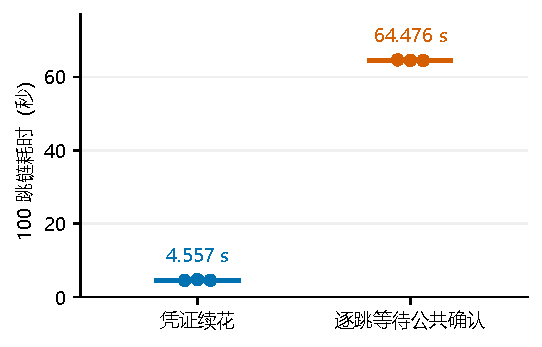
\includegraphics[width=\columnwidth]{continuation-final-zh.pdf}
  \caption{构建 721800c 的 100 跳链：每种模式三次运行，成员同步、钱包 NoSync。两种模式都终止于最后一次已认证接收；只有等待模式要求在跳间进行公开观察。}
  \label{fig:continuation}
\end{figure}

全部 297 个快速后继交易都使用其父交易的 TXCer，在父交易接收之后构造，并在四个副本中记录到的最早父交易应用提交完成之前首次发送。最小领先量为 224.785\,ms。这些记录标记的是数据库提交的时间，而非共识决定的时间。之后的驱动观测并不是原始的钱包验证时间戳。实际的缺失输入记录（而非发送顺序）确立了 3、2 和 4 次子交易先于来源交易执行，且全部在无赔付的情况下被履行。

驱动程序每 5\,ms 轮询一次，跟随者每 25\,ms 轮询一次；250\,ms 是提交设置。在每次等待运行的 99 次跳间等待中，从最早副本应用提交到驱动观测的总计为 29.542、29.681 和 29.347\,s。该联合区间包含后继区块头的可用性、获取、验证、本地记录以及副本差异。钱包内部的时间戳不能区分这些项。因此，14.15 是所测得的端到端模式之比，而非纯粹的共识加速或轮询惩罚。补充材料给出了匹配的区间以及从观测到下一次构造的时间。

快速模式的中位数为：最后一笔支付的公开观测 5.228\,s，所有支付的公开观测 5.229\,s，所有支付的成员闭合 5.294\,s。全部 600 笔支付都通过输入/输出、副本一致、CAL/FUEL、费用闭合和发件箱审计。每条链花费 9,400\,FUEL：8,400 为奖励，1,000 被销毁。对于这一固定形态，TXCer 大小为 779\,B；请求最初为 1,979\,B，此后为 2,766\,B，没有随祖先增长的情形。

\subsection{混合负载下的来源解决}
\label{sec:eval-mixed}
\label{sec:eval-liabilities}
\label{sec:eval-repair}

四个委员会进程与两个组织（每个组织有四名成员和一个网关）构成 14 个服务。费用使用明确授权的由组织支付的 FUEL。普通钱包为 NoSync；场景钱包同步提交，并在每种处理中跟随区块至少 55\,s。每次运行提供 7,000 笔独立的普通支付，目标为 100 笔/s 持续 70\,s，限制为 64 个快速请求与 256 笔未完成支付。从驱动程序启动后十秒开始，八个独立的跨组织父--子对以一秒间隔依次启动，所用输入与 Intent 与普通流相分离。每种处理都包含这些对。

N 正常交付。R 扣留每个已认证父交易的发布者提交与 INSTALL，并保持公开证据恢复启用。C 使用相同的扣留，但禁用恢复。P 另外暂停所有适配端点，但不暂停共识或决定。C/P 在观察到各自的赔付之后释放每个迟到的父交易，不等待另一个目标或表示。P 仅在全部四个副本报告全部八个目标均为 Recovered、且表示既未提交也未物化之后，才恢复适配。每种处理有三次全新运行，顺序为 N/R/C/P、P/C/R/N、N/R/C/P。

\begin{table*}[t]
  \caption{混合负载下的普通支付测量。每种处理有三次运行，每次含 7,000 笔普通支付外加八个父--子对。表项为运行级统计量的中位数，最后一列除外，该列为各次运行中最大的调度滞后 P95。发送跨度与排空自实际发送起测量；排空是一项观测。}
  \label{tab:eval-mixed}
  \centering
  \small
  \setlength{\tabcolsep}{7pt}
  \begin{tabular}{@{}lrrrrrr@{}}
    \toprule
    处理 &
    \shortstack{接收 P50\\(ms)} &
    \shortstack{接收 P95\\(ms)} &
    \shortstack{接收 P99\\(ms)} &
    \shortstack{发送跨度\\(s)} &
    \shortstack{发送后排空\\(s)} &
    \shortstack{最大调度 P95\\(ms)} \\
    \midrule
    N & 55.13 & 152.77 & 243.87 & 70.245 & 1.015 & 255.40 \\
    R & 53.03 & 139.89 & 220.06 & 69.990 & 0.890 & 0.24 \\
    C & 54.01 & 136.49 & 227.58 & 70.395 & 1.029 & 700.33 \\
    P & 55.00 & 144.21 & 227.52 & 70.576 & 1.155 & 895.88 \\
    \bottomrule
  \end{tabular}
\end{table*}

\noindent\textbf{适配不可用期间的经济闭合。}
R 自动履行全部 24 个被扣留的来源，无需发布者重新提交或赔付。在这些目标上，来源执行在子交易发送之后 2.054--3.357\,s 被观察到（中位数 2.905\,s）。C/P 对 48 个目标各赔付 100\,CAL，并回收每笔扣减：4,800\,CAL 被赔付并被偿还。在这 48 个目标上，赔付观测出现在子交易发送之后 31.806--34.499\,s，其中包括 30 秒的公开时间截止期、调度、执行和轮询。

在 P 中，全部 96 次副本--目标检查都在适配恢复之前确认了偿还，时间为第一笔普通发送之后 51.256--51.792\,s。随后的每个表示与物化都在最后一笔普通发送之前完成。这一顺序在所测的执行中展示了适配不可用时的经济闭合（图~\ref{fig:mixed-load}），而不是由最终余额相符来推断其独立性。

\begin{figure*}[t]
  \centering
  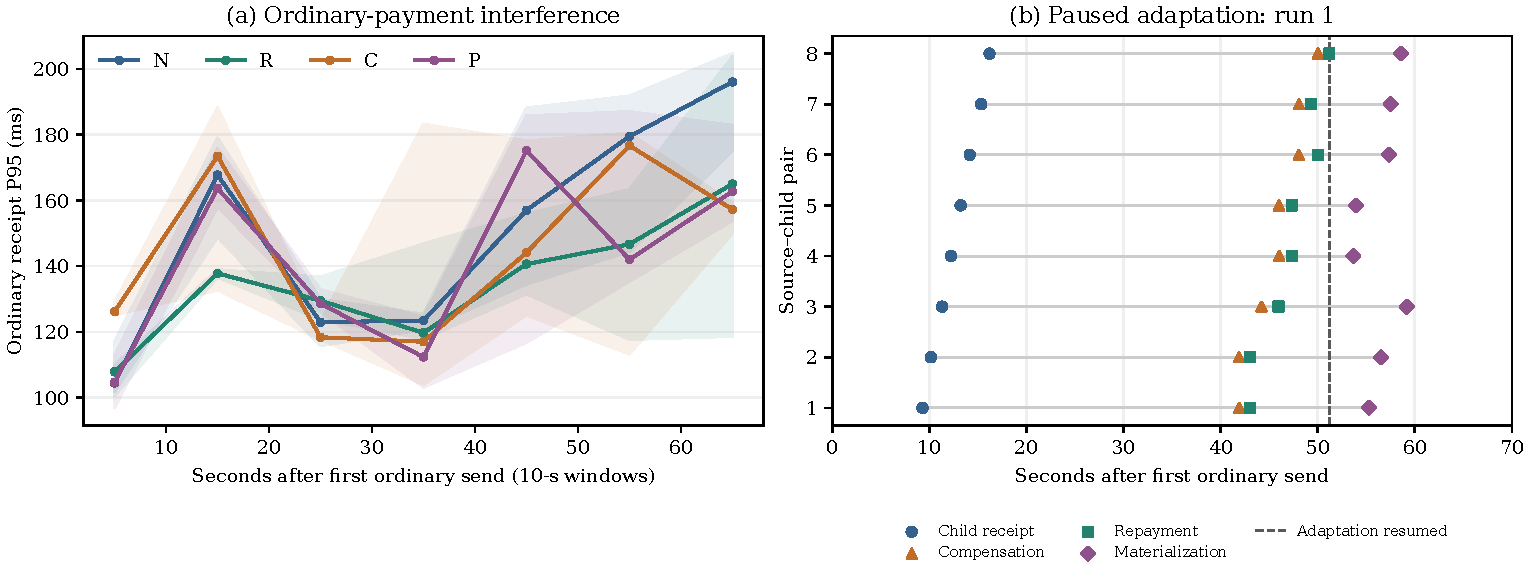
\includegraphics[width=\textwidth]{mixed-load.pdf}
  \caption{混合负载观测。左：前七个十秒窗口中的普通接收 P95；线为三次运行的中位数，带为最小值--最大值，而非置信区间。右：P 第 1 次运行中的八个目标，展示适配恢复之前的赔付与偿还以及随后的物化。公开事件是观测，而非内部提交时间戳。}
  \label{fig:mixed-load}
  \label{fig:c3-resolution}
\end{figure*}

\noindent\textbf{共享资源代价与审计。}
表~\ref{tab:eval-mixed} 同时报告被接纳的接收延迟与实际发送跨度及排空。所有 N/C 运行和两次 P 运行都达到 256 个未完成的上限；两次 C 运行和两次 P 运行还达到 64 个快速请求。从计划发送到实际发送所测得的调度滞后，其运行级 P95 达到 895.88\,ms。P 第 1 次运行在 70\,s 之后的尾部含 89 笔支付，接收 P95 为 282.61\,ms；它不是完整的十秒窗口。因此较低的汇总分位数并不能确立性能改进或零干扰。所有运行都在最后一笔普通发送之后 0.815--1.356\,s 排空。

十二次运行中的全部 84,192 笔支付都闭合。每次运行的四个副本在同一高度一致；CAL/FUEL 守恒、费用、身份、义务和发件箱均通过审计。各处理之间最终的用户 CAL 分配一致，备付金得以恢复，CAL/work 预留清空且无预算拒绝。N/R 每次运行花费 659,504\,FUEL；C/P 花费 659,544，其中包括八笔额外的 5-FUEL 赔付费用。实际花费的费用不会被恢复为可用资金。

在聚合之前逐笔计算的归档计划到接收 P95，对 N/R/C/P 分别为 304/140/475/667\,ms。这包括发送前的背压；补充材料将时间戳约定以及少量墙钟异常与实际发送接收延迟分开记录。

\subsection{历史读取：等价的答案与明确的代价}
\label{sec:eval-reader}

读取者是已验证并执行前缀 $H$ 的诚实本地副本，在一个应用读事务 $V_H$ 内查询原始坐标 $(h,j,k)$。A 加载原始历史并使用永久决定索引；B 使用既有的 Canonical 修订。二者查阅相同的永久决定与义务，在 $H$ 处返回相同的输入身份、TxID、坐标、金额、历史资金/扣减、决定/高度以及义务状态。授权来自绑定确切修订的成功执行，而不是 CH 等式或匹配的 BlockID。这不是远程服务器认证。

测试夹具使用真实签名、成功的 ABCI 执行、基于磁盘的 bbolt/GoLevelDB 以及冻结的 BlockStore。A 拥有自己的原始 BlockStore，不含 B 的备份布局代价。点查询加载一个区块并解码所选交易；A 的区块查询扫描其范围索引一次并构建一个计时的映射。两种策略都不会获得预先计算的决定映射。页面是热的，没有已解码区块或结果缓存；\texttt{GOMAXPROCS=16}，\texttt{GOGC=100}。

三个全新进程各测试四个 $(n,m)$ 夹具，其中 $n\in\{32,256\}$ 为支付数，$m\in\{1,8\}$ 为每个区块的已赔付槽位数。每种策略 20 次预热之后，对已赔付点、普通点和整区块各做每种策略 300 次交错查询，共得到 21,600 次计时查询。计时包含读事务边界、加载/解码、记录关联和结果构造。所有计时读取都使用已表示且已物化的 $H=4$；其他阶段以及随后的真实偿还属于功能等价性检查，而非额外的计时样本。

\begin{table*}[t]
  \caption{历史读取与表示的代价。A 为原始历史加决定索引；B 为 Canonical。点读取以已赔付槽位为目标。查询表项为三个运行级 P50 的中位数；代价表项为三个总量的中位数。额外 KV 不含公共历史、决定和应用提交元数据。}
  \label{tab:eval-reader}
  \centering
  \small
  \setlength{\tabcolsep}{8pt}
  \begin{tabular}{@{}crrrrrr@{}}
    \toprule
    $(n,m)$ &
    \multicolumn{2}{c}{点读取 ($\mu$s)} &
    \multicolumn{2}{c}{整区块 ($\mu$s)} &
    \shortstack{额外净 KV\\(MiB/区块)} &
    \shortstack{本地工作\\(ms/区块)} \\
    \cmidrule(lr){2-3}\cmidrule(lr){4-5}
    & A & B & A & B & & \\
    \midrule
    $(32,1)$  & 162.54  & 148.38 & 1,028.29 & 1,005.79 & 0.279 & 43.32 \\
    $(32,8)$  & 169.21  & 156.62 & 1,127.46 & 1,083.71 & 0.314 & 94.46 \\
    $(256,1)$ & 1,005.21 & 881.38 & 8,441.58 & 8,316.00 & 2.153 & 65.32 \\
    $(256,8)$ & 1,006.25 & 887.25 & 8,554.17 & 8,407.12 & 2.189 & 214.40 \\
    \bottomrule
  \end{tabular}
\end{table*}

Canonical 使已赔付点的 P50 降低 7.44--12.32\%（12.6--123.8\,$\mu$s）；整区块的差异为 1.49--3.88\%（表~\ref{tab:eval-reader}）。在 $(256,8)$ 第 1 次运行中，A 执行 12 次 BlockStore Get，返回 622,183\,B；B 不执行任何 Get，但从应用状态读取 825,526\,B。每次查询的平均堆分配约为 4.95 对 2.24\,MB，而记录关联的中位数为 11.50 对 10.83\,$\mu$s。这表明的是布局/重建方面的收益，而不是更少的总字节数或密码学加速。解码对象缓存可能改变这一权衡。

表示为每个被修复的区块增加 0.28--2.19\,MiB 的净逻辑 KV，用于修订、任务以及备份/历史记录，已扣除被删除的 Pending。$(256,8)$ 的 5,056-B 批次已包含在内。本地顺序适配、组装、Finalize、同步的应用 Commit 与物化合计 43--214\,ms。它不含网络/共识等待、公开区块保存以及提交签名的构造。公共的赔付成本另行报告。

等价性检查涵盖：先赔付后表示、先表示后物化，以及偿还时保留历史扣减且状态为 Recovered。无效坐标、跨前缀决定以及错误的扣减/金额都被拒绝；无法解码的修订会失败而不回退。这些检查并不确立对任意可解码的损坏的检测。Canonical 在稳定的历史坐标处提供授权的资金表示，并带有所测得的维护代价，而不是一个经济上必需的、或普遍更快的索引历史替代方案。

\subsection{注入延迟与单故障运行}
\label{sec:eval-faults}
在 \texttt{9879f64} 上，四种条件各运行三次，顺序交替。H 使用注入代理但不增加延迟；L 对成员 RPC 与委员会 P2P 流量每方向增加 25\,ms。L-M 与 L-C 增加该延迟，并分别在 15 至 45\,s 暂停成员~3 或委员会验证者~3。每次运行发送 100 笔预热支付、1,200 笔 20/s 的普通支付，以及两条在故障窗口内启动的 10 跳链。实际的健康检查 RPC RTT 从 1.17 升至 52.20\,ms；RPC 与 P2P 的平均保持时间均约为每方向 25.2\,ms。补充材料规定了 FIFO 注入、固定资源和逐次运行的结果。

全部 15,840 笔支付均闭合，委员会状态相等，发件箱为空，公开缺口为零。无需赔付。表~\ref{tab:eval-faults} 区分了接收、公开观测以及对全部四名成员的观测。暂停一名成员时，新的 QC 使用其余三名成员，公开完成继续进行，而缺席成员的观测造成 630--641 个未完成任务的峰值。暂停一名验证者时，接收 P95 保持在 108--111\,ms，每个故障窗口内有 400--510 笔支付达到公开观测，但公开 P95 升至 9.5--12.6\,s。保留的提交证书验证了每次运行中暂停验证者的五次第 0 轮提议者机会；每次都在第~1 轮提交，且不含该验证者的签名。两条链均在各自故障窗口内完成认证，且每次运行都在其最后一笔普通发送之后 1.25\,s 内排空。这些是单机注入延迟的结果，与 fast/wait 对比相互独立。

\begin{table}[t]
\caption{注入延迟与单故障：每次运行全部 1,200 笔普通支付的三个运行级统计量的中位数；预热与链不计入。公开与成员列为发送到观测的 P95；成员列等待全部四名成员。}
\label{tab:eval-faults}
\centering\small
\begin{tabular}{@{}lrrr@{}}
\toprule
条件 & 接收 P50/P95 (ms) & 公开 (s) & 成员 (s)\\
\midrule
H   & 41.56/83.20  & 1.28 & 1.36\\
L   & 81.91/118.22 & 1.32 & 1.41\\
L-M & 77.71/112.85 & 1.30 & 29.00\\
L-C & 77.41/109.32 & 10.02 & 10.04\\
\bottomrule
\end{tabular}
\end{table}


\subsection{当前构建的边界与组合检查}
\label{sec:eval-boundaries}
\texttt{9879f64} 上的确定性测试使用实际的成员批准、ABCI 执行和经认证的跟随者更新。它们复现了无 QC 的额度碎片化、同输入 2/2 分裂，以及带完整 CAL/FUEL 核算的两轮 Intent 冲突赔付。外部充值解决了第一种情形，而不能解决第二种。真实的门限适配涵盖两种表示/偿还顺序；保留状态的重启复现每个原始命令历史。提交后、签名返回之前的中断保留锁与预留，并允许幂等重试。补充材料给出了逐前缀的账本、负向入口测试和重启断言。

\noindent\textbf{归档证据。}
补充材料保留了较早的继续、吞吐量、资本、组织路径和可用性实验，其构建与配置均保持原样。它们提供的是历史背景，而不是对 \texttt{721800c} 的测量；跨版本的差异不归因于个别改动。

\section{结论}
\label{sec:conclusion}

Next 让收款方能够依据已认证的证据继续花费，同时由一个明确的、有备付金支撑的签发组织对每一个缺失的源交易负责。在基线版本上，100 跳链完成最后一次认证接收的用时中位数为 158.846\,ms，而在各跳之间等待公共确认则需要 65.204\,s；九轮实验关闭了 21,600 笔支付，并偿还了全部 216 次赔付。另外两项性质规定了缺失来源如何关闭。第一，延迟只改变备付金的临时占用：当所有源交易都执行时，到达与赔付的任意顺序最终得到相同的最终持有者。第二，赔付决定是一条只需要委员会的公共记录；随后把该扣减记录进已存储区块的历史表示路径可以滞后或停止，而不妨碍义务关闭。decision-first 实验印证了这一点：在全部四个适配服务暂停时，赔付与偿还仍然完成，并且被扣留的源交易通过原签署者的补交得以执行。这些路径将支付续花与来源交付分离，并将经济关闭与历史物化分离。

\section*{致谢}
ChatGPT 与 Claude 辅助起草和修订摘要、正文及中文阅读版；Codex 辅助基于源码的审阅、修订、LaTeX 组装与绘图脚本。实验图表由所记录的测量数据生成。

\bibliographystyle{IEEEtran}
\bibliography{references}
\end{document}
